\documentclass{ieeetj}
\newcommand{\seclogo}{}
\usepackage{cite}
\usepackage{amsmath,amssymb,amsfonts}
\usepackage{listings}
\usepackage{algorithmic}
\usepackage{graphicx,color}
\usepackage{textcomp}
\usepackage{xcolor}
\usepackage{hyperref}

\hypersetup{hidelinks=true}
\usepackage{algorithm,algorithmic}
\lstset{
    language=Java,
    basicstyle=\ttfamily\small,
    keywordstyle=\bfseries\color{blue},
    stringstyle=\color{red},
    morecomment=[l][\color{magenta}]{//},
    frame=single,
    breaklines=true,
    showstringspaces=false,
    tabsize=1,
}
\def\BibTeX{{\rm B\kern-.05em{\sc i\kern-.025em b}\kern-.08em
    T\kern-.1667em\lower.7ex\hbox{E}\kern-.125emX}}
\AtBeginDocument{\definecolor{tmlcncolor}{cmyk}{0.93,0.59,0.15,0.02}\definecolor{NavyBlue}{RGB}{0,86,125}}

% Definim el logo
\def\OJlogo{
    \vspace{-14pt} % Espai negatiu per pujar el logo
    
\includegraphics[height=0.96cm]{png/logo.png}}

\begin{document}
\receiveddate{25 Febrer, 2025}
\publisheddate{21 Març, 2025}
\currentdate{25 Març, 2025}

\title{Dividir'N'Vencer: Càlcul de Distàncies Extremes en Núvols de Punts 2D i 3D amb "Divideix i Venceràs"}

\author{Josep Ferriol, Daniel García, Khaoula Ikkene, Biel Perelló} \affil{Universitat de les Illes Balears, Departament d'Enginyeria Informàtica} \corresp{Autor de contacte: Daniel García (email: daniel.garcia19@estudiant.uib.es)}

\begin{abstract} 
Aquest document presenta el desenvolupament d’una aplicació per al càlcul de distàncies entre punts dins un núvol bidimensional, o tridimensional, generat de manera aleatòria. L’objectiu principal ha estat implementar dues estratègies per determinar la parella de punts més propera: una solució bàsica amb cost asimptòtic \( O(n^2) \), basada en la comparació exhaustiva de totes les possibles parelles, i una solució optimitzada amb cost \( O(n \log n) \), basada en el paradigma Divideix i Venceràs \cite{DivideAndConquer}. Com a extra s'ha implementat la distancia mínima amb un KD-Tree \cite{kdTree}. 

A més, s’han desenvolupat algorismes eficients per determinar la parella de punts més allunyada dins el conjunt (convex hull i l'uniforme), i s’ha realitzat una comparació empírica del rendiment dels diferents mètodes implementats per diversos valors de \( N \), mesurant-ne tant el temps d’execució com l’escalabilitat. L’aplicació ha estat implementada emprant Java i seguint l’arquitectura Model-Vista-Controlador (MVC), que ha permès separar clarament la lògica de càlcul, la interfície gràfica i el control dels esdeveniments \cite{SwingLibrary}, \cite{MVCPattern} \cite{JavaFX}.

Finalment, s’han utilitzat diferents funcions de distribució (uniforme, gaussiana, exponencial) per a la generació aleatòria dels punts, amb l’objectiu d’analitzar la robustesa dels algoritmes en escenaris estadísticament diversos.
\end{abstract}

\begin{IEEEkeywords} 
Algorismes de Divisió i Conquesta, Arquitectura de Programari, Càlcul de Distàncies, Cost Asimptòtic, Java Swing, Model-Vista-Controlador, Núvols de Punts, Programació Recursiva
\end{IEEEkeywords}


\maketitle

\section{Introducció} 
Aquest projecte té com a objectiu implementar diversos algorismes per calcular la distància entre punts dins un núvol bidimensional generat de forma aleatòria, aplicant una arquitectura MVC. En particular, es pretén determinar tant la parella de punts més propera com la més allunyada, mitjançant estratègies d’eficiència diferent, i analitzar-ne el comportament segons la complexitat computacional i l’escenari de generació dels punts \cite{closestPairTheory}.

El Model Vista Controlador (MVC) és un patró d'arquitectura de programari àmpliament utilitzat per separar la presentació de dades, la gestió de dades i la lògica del programa. Aquesta separació permet millorar la modularitat i mantenibilitat dels sistemes, facilitant així el desenvolupament i manteniment de les aplicacions \cite{MVC_Theory}.

En aquesta memòria, es presenten els conceptes teòrics de l'arquitectura MVC, incloent la seva estructura i els avantatges que ofereix \cite{mvcBenefits}. També s'explica el patró per esdeveniments, que permet una comunicació eficient entre els components del sistema mitjançant la gestió d'esdeveniments i notificacions.

A continuació, es descriu l'entorn de programació utilitzat per al desenvolupament de l'aplicació, incloent les llibreries de Swing per a la interfície gràfica i les eines emprades per a la gestió del codi i el control de versions \cite{SwingLibrary}.

La part central de la pràctica consisteix en desenvolupar una aplicació que implementi dues estratègies per al càlcul de la parella de punts més propera: una solució bàsica amb complexitat \( O(n^2) \), basada en un doble bucle que compara totes les parelles possibles, i una solució més eficient basada en Divideix i Venceràs amb cost \( O(n \log n) \). A més, es dissenya i implementa un mètode per trobar la parella de punts més allunyada del conjunt. Totes aquestes funcionalitats són accessibles a través d’una interfície gràfica desenvolupada amb Java Swing, que permet també modificar diversos paràmetres del problema, com el nombre de punts o la distribució emprada per generar-los.

Finalment, s'analitzen els resultats obtinguts i es presenten les conclusions del projecte, incloent la comparació empírica entre estratègies, l’impacte de les distribucions estadístiques utilitzades i propostes de millora, com la incorporació de paral·lelisme, algorismes basats en estructures de dades avançades o l’extensió a espais tridimensionals.


\subsection{Model Vista Controlador (MVC)}
El patró arquitectònic Model Vista Controlador (MVC) és una estratègia de disseny que divideix una aplicació en tres components ben diferenciats: el Model, la Vista i el Controlador. Aquesta divisió facilita una millor organització del codi i permet un desenvolupament més modular, mantenible i escalable \cite{MVC_Theory}.

\begin{itemize}
    \item \textbf{Model}: Representa l'estat intern de l'aplicació i encapsula tota la lògica relacionada amb les dades. En el context d’aquesta pràctica, el model s'encarrega de generar el conjunt de punts aleatoris, calcular les distàncies entre parelles de punts i emmagatzemar els resultats rellevants.
    
    \item \textbf{Vista}: És el component encarregat de mostrar la informació a l'usuari. Aquesta vista es materialitza mitjançant una interfície gràfica d'usuari (GUI), que visualitza el núvol de punts, les parelles més properes i més allunyades, i proporciona opcions d’interacció com el nombre de punts o el tipus de distribució.
    
    \item \textbf{Controlador}: Actua com a enllaç entre la Vista i el Model. Rep les accions de l’usuari, com per exemple la petició de generar un nou núvol o calcular distàncies, i delega les tasques corresponents al Model. Un cop el Model ha actualitzat les dades, el Controlador s'encarrega de notificar la Vista per reflectir els canvis.
\end{itemize}

En aquest projecte, l’ús del patró MVC no només contribueix a una millor estructuració de l’aplicació, sinó que també permet una separació clara de responsabilitats: la generació i càlcul de dades romanen totalment independents de la seva visualització. Això facilita, per exemple, substituir la Vista per una diferent (com una API REST o una altra llibreria gràfica) sense afectar el nucli de càlcul, o bé canviar l’algorisme sense alterar la presentació.

\begin{figure}[htbp]
    \centerline{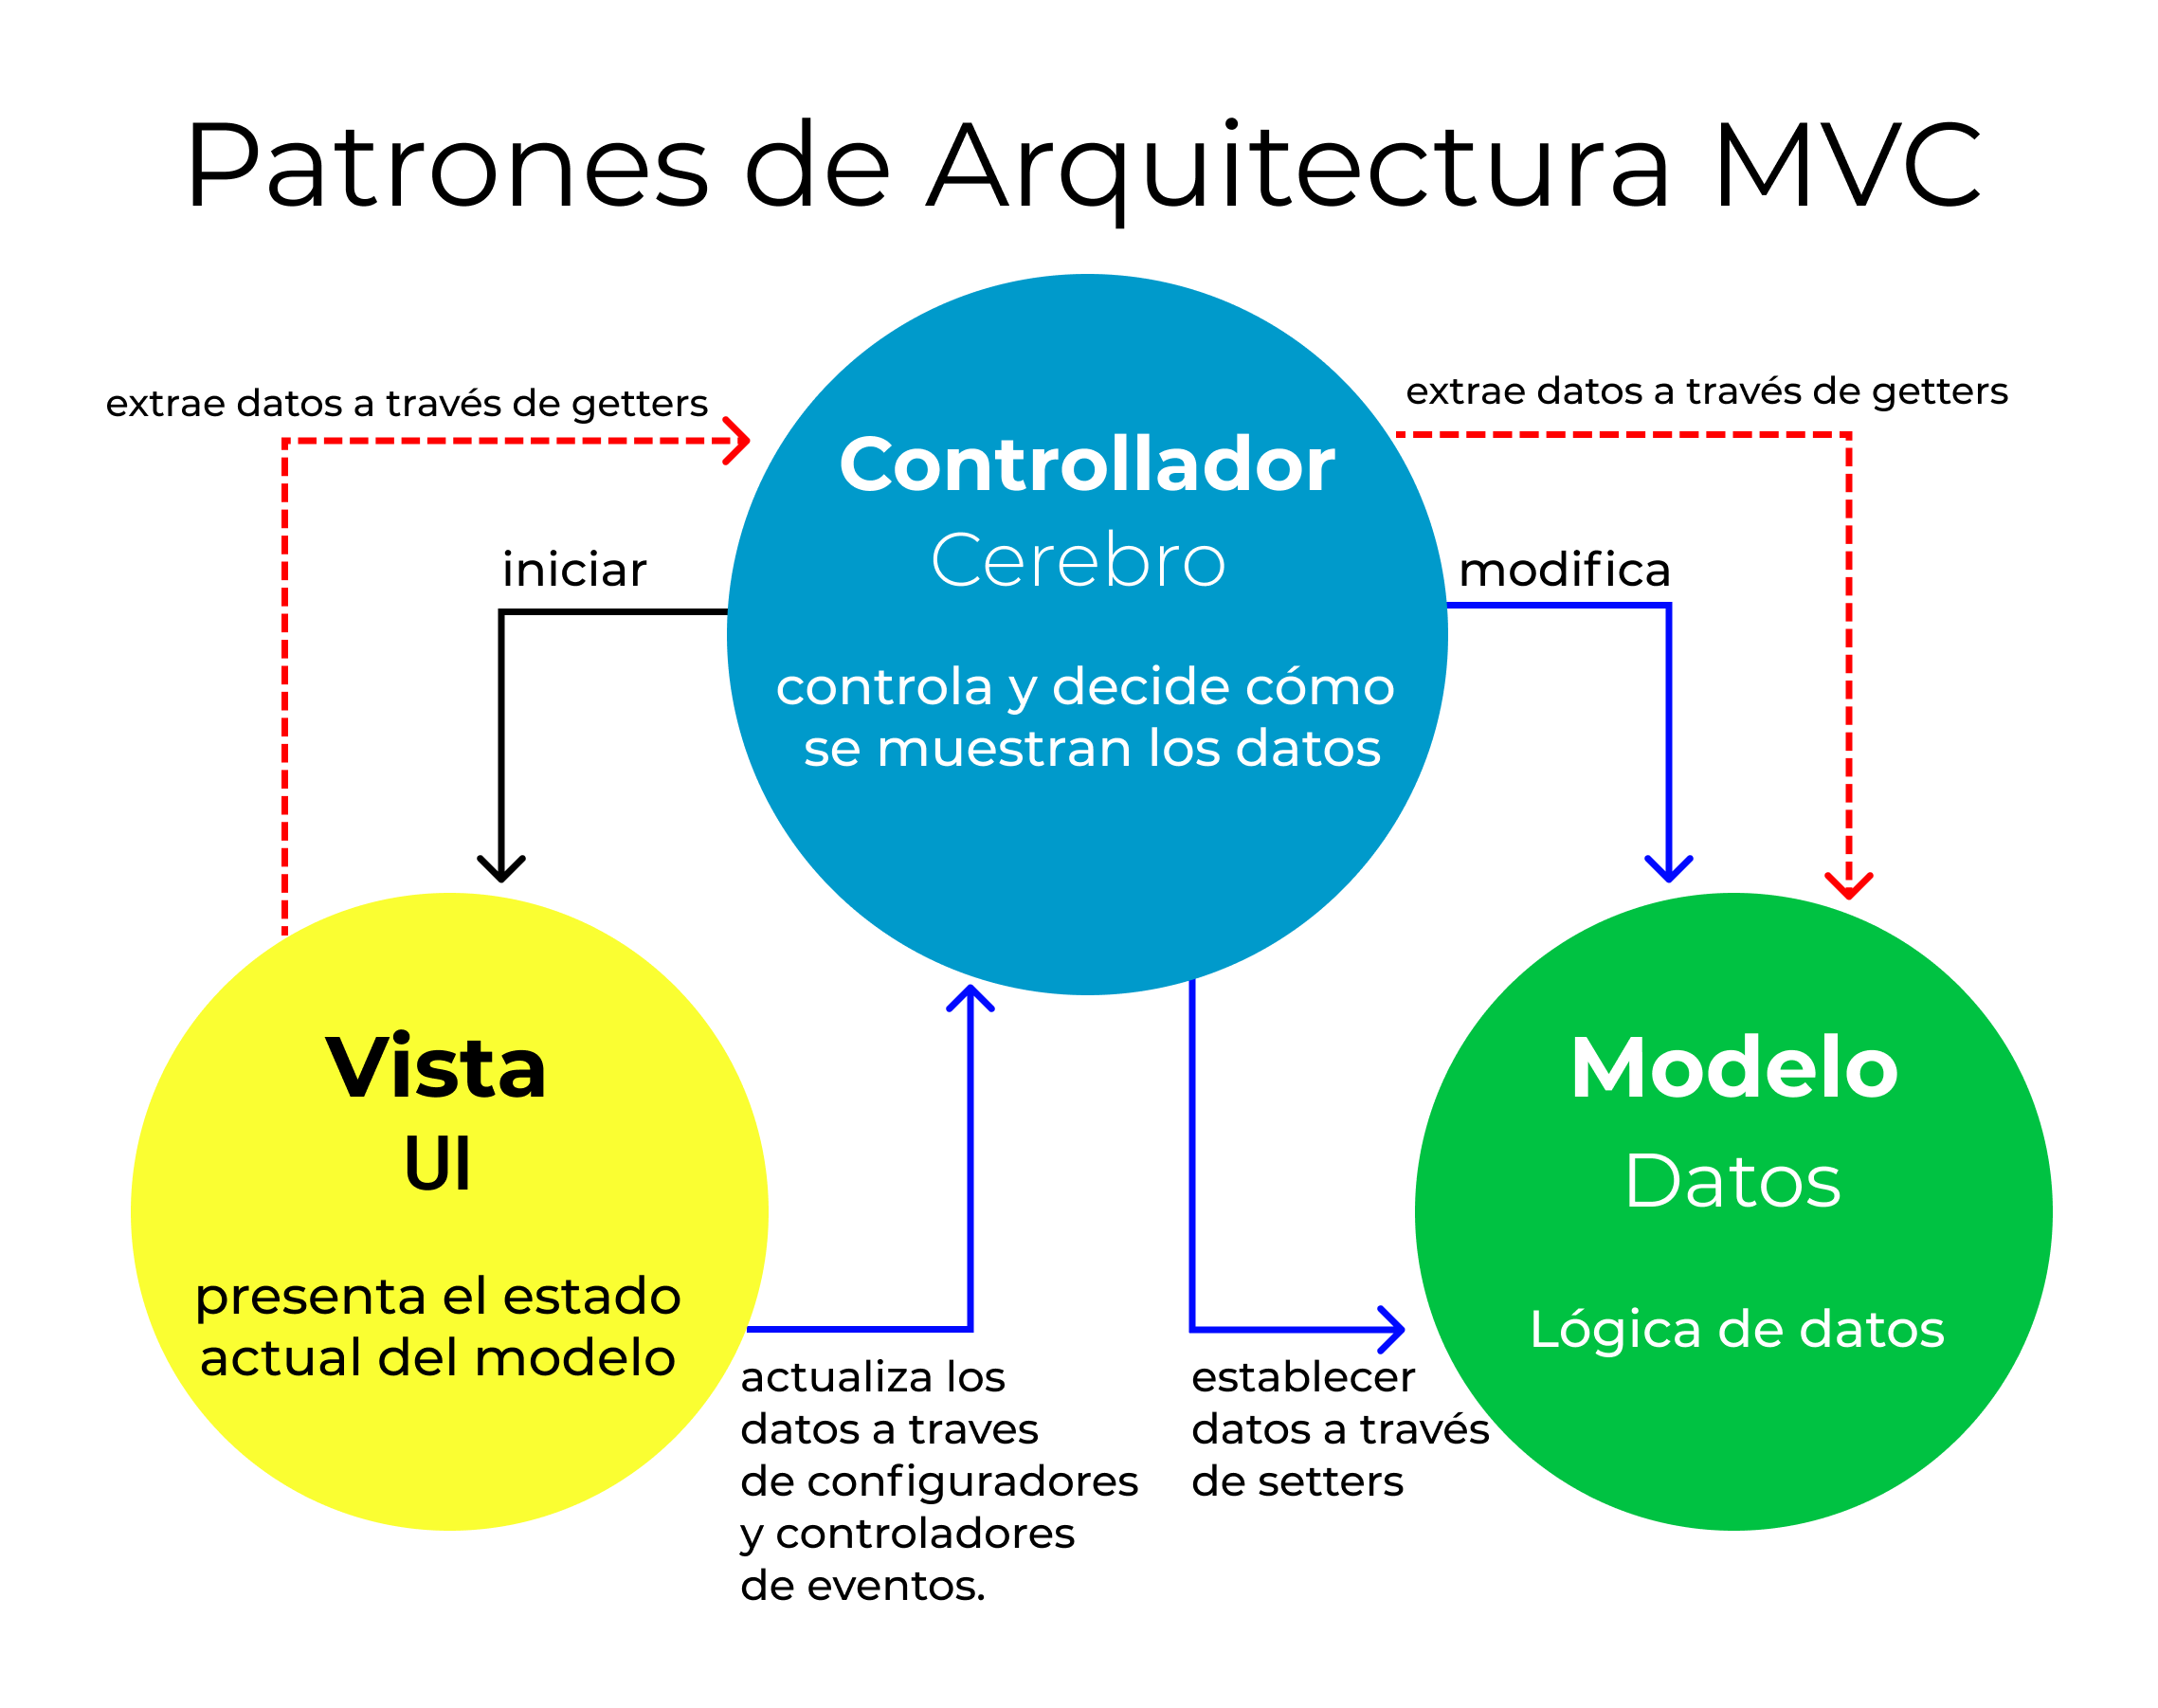
\includegraphics[width=0.4\textwidth]{png/mvc.png}}
    \caption{Arquitectura MVC aplicada a l’aplicació.}
    \label{fig:mvc-nuvol}
\end{figure}

El patró va ser concebut inicialment per Trygve Reenskaug a la dècada dels 70, i des d’aleshores ha esdevingut un dels enfocaments més utilitzats en el desenvolupament de sistemes interactius. Un dels seus avantatges principals és que permet que diversos desenvolupadors treballin de manera paral·lela en diferents components sense generar conflictes entre ells.

En definitiva, MVC resulta especialment útil en entorns acadèmics i professionals on es prioritza la claredat estructural i la reutilització del codi. En el marc d’aquesta pràctica, l’arquitectura ha estat fonamental per garantir una implementació neta, clara i extensible de la funcionalitat de càlcul i visualització de distàncies entre punts.

\subsection{Patró per Esdeveniments}
El patró per esdeveniments és una estratègia de disseny que facilita la comunicació entre components d'una aplicació de forma desacoblada, mitjançant la generació i gestió d'esdeveniments \cite{Patró per Esdeveniments}. Aquest enfocament és especialment útil en interfícies gràfiques, on l'aplicació ha de reaccionar a interaccions de l’usuari de manera asíncrona i eficient.

\begin{itemize}
    \item \textbf{Emissió d’esdeveniments}: Quan un component detecta una acció rellevant —com ara una interacció de l’usuari— pot emetre un esdeveniment per notificar a altres components que s’ha produït un canvi d’estat o una acció concreta. En aquesta pràctica, per exemple, quan l’usuari prem un botó per generar punts o calcular distàncies, la Vista emet un esdeveniment que el Controlador captura per iniciar el procés de càlcul.
    
    \item \textbf{Recepció i maneig}: Altres components poden escoltar (subscripció) aquests esdeveniments per executar una acció determinada quan es produeixin. El Controlador, en aquest cas, actua com a receptor dels esdeveniments generats per la Vista, coordinant la invocació al Model per realitzar els càlculs i actualitzant posteriorment la Vista amb els resultats obtinguts.
    
    \item \textbf{Desacoblament dels components}: L’ús del patró per esdeveniments proporciona una arquitectura més flexible, ja que els components no necessiten tenir referències directes entre ells. Això facilita la reutilització del codi i simplifica la integració de noves funcionalitats. A tall d’exemple, seria possible substituir la Vista per una nova implementació sense modificar la lògica del Model, mantenint intacta la comunicació a través dels esdeveniments.
\end{itemize}

L'aplicació del patró per esdeveniments resulta especialment rellevant quan es treballa amb entorns gràfics i processos asíncrons, com en aquesta pràctica, on les interaccions de l’usuari poden produir múltiples accions consecutives o simultànies. Aquest mecanisme permet mantenir una arquitectura robusta, modular i fàcilment escalable.

\subsection{Càlcul del Cost Asimptòtic}
L’anàlisi del cost asimptòtic permet avaluar el rendiment dels algorismes segons la seva eficiència temporal i espacial, especialment quan es treballa amb conjunts de dades grans. Aquesta anàlisi es realitza mitjançant la notació Big-O, que proporciona una estimació de com creix el temps d’execució en funció de la mida de les dades d’entrada, \(n\) \cite{bigOAnalysis}. La notació Big-O s’enfoca en el comportament en el pitjor cas i ignora constants i factors de menor ordre per oferir una visió general de l’escalabilitat d’un algorisme.

\begin{figure}[htbp]
\centerline{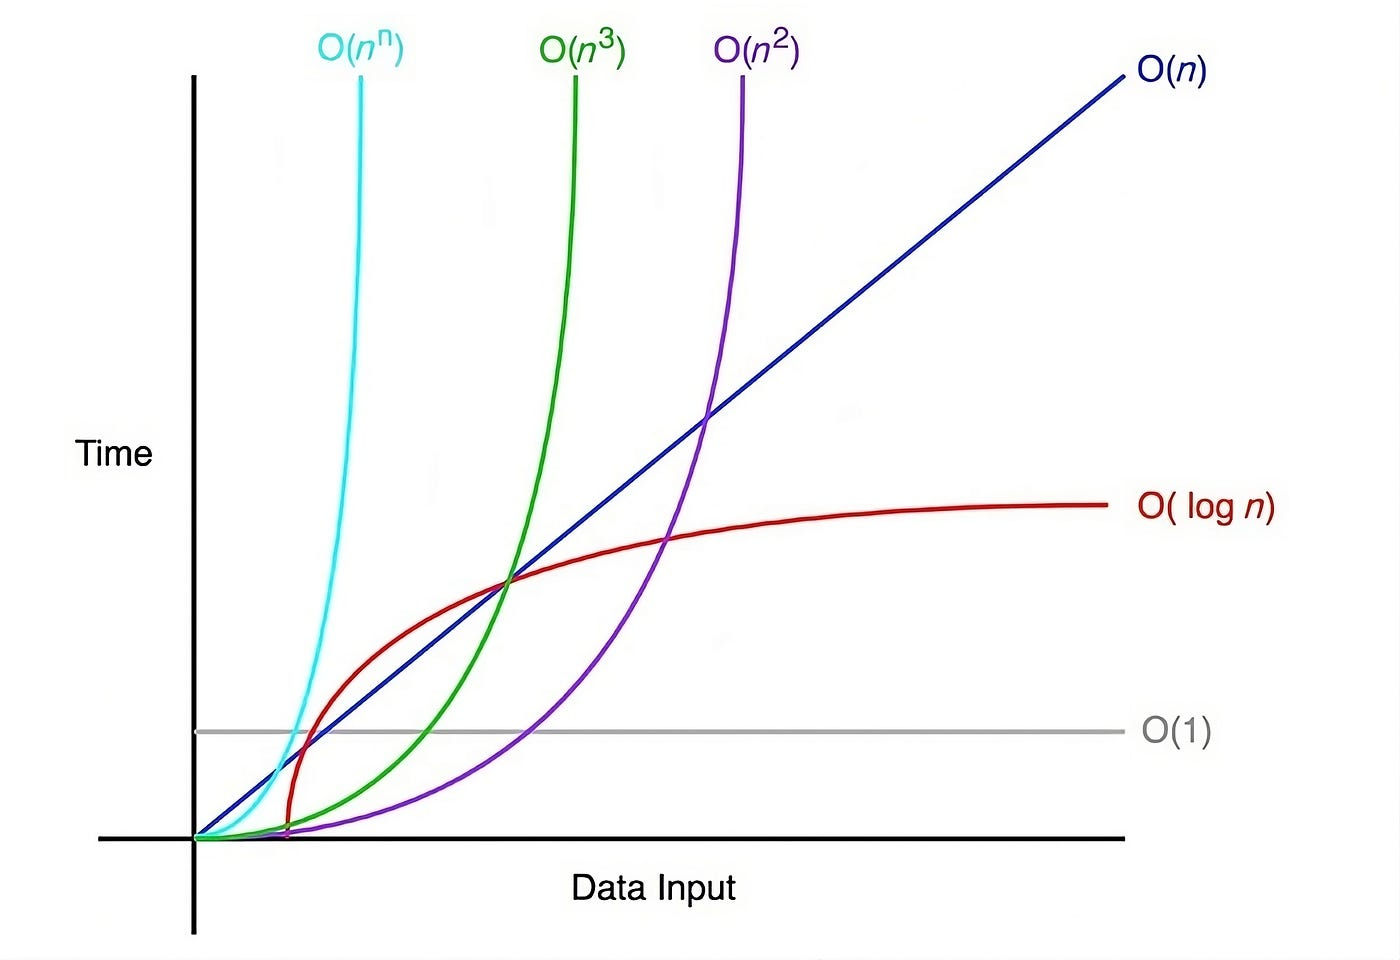
\includegraphics[width=0.45\textwidth]{png/bigO.jpg}}
\caption{Comparació entre diferents ordres de creixement segons la notació Big-O.}
\label{fig:big_o}
\end{figure}

En aquesta pràctica, centrada en el tractament i processament de núvols de punts, s’han identificat dues complexitats principals:

\begin{itemize}
    \item \textbf{\(O(n^2)\)}: Aquesta complexitat apareix en algorismes que requereixen comparar cada punt amb tots els altres, com pot ser el càlcul exhaustiu de totes les distàncies entre parelles de punts. Aquest enfocament pot ser costós quan el nombre de punts augmenta significativament.
    \item \textbf{\(O(n \log n)\)}: Present en algorismes que impliquen ordenació, o bé estratègies més eficients per trobar parelles pròximes de punts. Per exemple, en lloc de comparar totes les parelles possibles, es poden aplicar tècniques com l’ordenació espacial (divisió i cerca) que redueixen considerablement el cost computacional respecte a l’enfocament quadràtic.
\end{itemize}

Aquestes dues complexitats s’analitzaran amb més detall en la secció de resultats, on es mostraran comparatives empíriques entre diferents enfocaments implementats. L’objectiu és evidenciar com l’elecció de l’algorisme afecta significativament el rendiment quan es treballa amb conjunts de dades de mida considerable.

\subsection{Estratègia Divideix i Venceràs}

L’estratègia \textit{Divideix i Venceràs} (\textit{Divide and Conquer}, D\&C) és una tècnica fonamental en el disseny d’algorismes que consisteix a resoldre problemes complexos descomponent-los en subproblemes més petits, resolent aquests recursivament, i finalment combinant les solucions parcials per obtenir la solució global del problema \cite{DivideAndConquer}. Aquesta tècnica ha demostrat ser extremadament eficaç en múltiples àmbits com la lògica, el disseny de programes modulars, els circuits digitals, i especialment en l’anàlisi d’algorismes d’ordenació i cerca.

\begin{itemize}
    \item \textbf{Dividir}: Es parteix el problema original en diversos subproblemes independents, habitualment de mida menor.
    \item \textbf{Vèncer}: Cada subproblema es resol de manera recursiva. Quan la mida del subproblema és prou petita, es resol directament (cas base).
    \item \textbf{Combinar}: Les solucions dels subproblemes es combinen per obtenir la solució del problema original.
\end{itemize}

\begin{figure}[htbp]
    \centerline{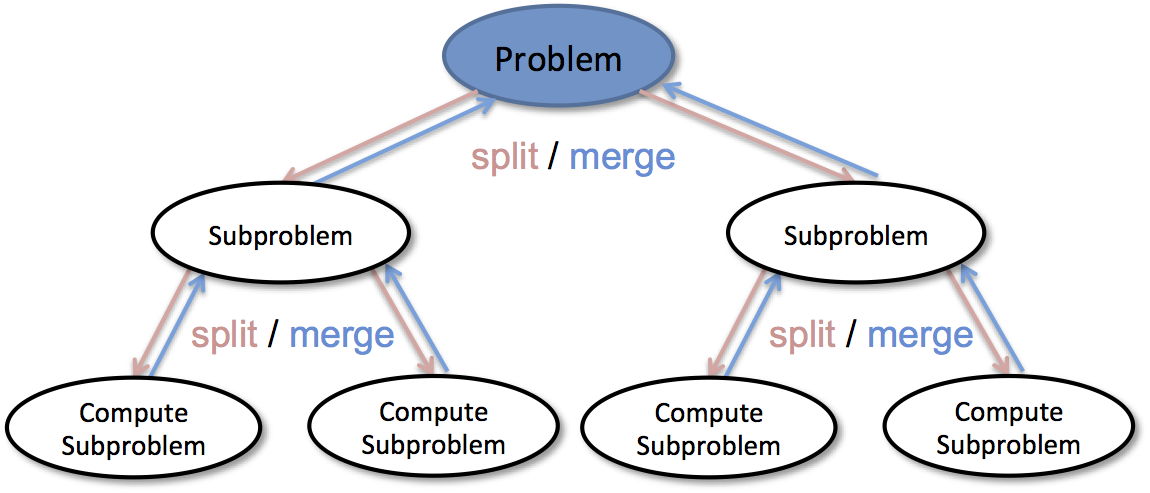
\includegraphics[width=0.4\textwidth]{png/DC.png}}
    \caption{Esquema de l'algoritme de Divide and Conquer.}
    \label{fig:divideANDconquer}
\end{figure}

Aquesta estratègia no es pot aplicar de manera universal. Perquè sigui eficient i viable, han de complir-se les condicions següents:

\begin{itemize}
    \item Ha d’existir una manera senzilla i eficient de resoldre els casos base.
    \item El problema ha de poder-se dividir fàcilment en subproblemes independents.
    \item Els subproblemes han de ser disjunts i no superposar-se.
    \item La combinació de les solucions parcials ha de tenir un cost inferior al de resoldre el problema de forma directa.
\end{itemize}

\textbf{Avantatges:}
\begin{itemize}
    \item Pot millorar considerablement la complexitat asimptòtica respecte a enfocaments iteratius o força bruta.
    \item Afavoreix el disseny modular i facilita la comprovació i manteniment del codi.
    \item És una tècnica naturalment recursiva i paral·litzable, cosa que permet l'execució concurrent en arquitectures multi-nucli.
\end{itemize}

\textbf{Desavantatges:}
\begin{itemize}
    \item Pot implicar un consum de memòria addicional degut a les crides recursives.
    \item El cost de la combinació pot arribar a ser elevat si no es dissenya adequadament.
    \item Pot ser menys eficient si els subproblemes no són realment independents o si la combinació no és trivial.
\end{itemize}

En aquesta pràctica, l’objectiu és trobar el parell de punts més propers dins d’un conjunt de punts generats aleatòriament en el pla. Una primera aproximació trivial seria calcular totes les distàncies entre parelles de punts, cosa que té una complexitat temporal de \(O(n^2)\). No obstant això, podem obtenir una millora significativa aplicant l’estratègia de \textit{Divideix i Venceràs}.

El procediment consisteix en:
\begin{enumerate}
    \item Ordenar prèviament els punts per la seva coordenada \(x\), amb un cost de \(O(n \log n)\).
    \item Dividir el conjunt per la meitat, formant dos subconjunts aproximadament iguals.
    \item Aplicar recursivament l’algorisme a cada subconjunt per trobar la distància mínima local.
    \item Combinar les dues solucions considerant la franja vertical propera a la línia divisòria i cercant-hi possibles parelles més properes entre punts de diferents subconjunts.
\end{enumerate}

Aquesta combinació s’efectua de manera eficient gràcies a propietats geomètriques que limiten el nombre de comparacions necessàries dins de la franja. Gràcies a això, l’algorisme global presenta una complexitat asimptòtica de \(O(n \log n)\), molt millor que el mètode exhaustiu de \(O(n^2)\).

L’estratègia de \textit{Divideix i Venceràs} no només permet millorar l’eficiència dels algorismes, sinó que aporta també una estructura lògica i modular al disseny del codi. En el context d’aquesta pràctica, s’ha demostrat especialment útil per reduir el cost computacional de la cerca del parell de punts més propers, i serveix com a exemple representatiu de l’impacte que pot tenir una bona elecció d’estratègia algorísmica en el rendiment global d’una aplicació.

\subsection{Núvols de Punts en l'Espai euclidià}

Un \textit{núvol de punts} és una col·lecció finita de punts definits dins d’un espai euclidià, generalment representats per coordenades \((x, y)\) en dues dimensions, \((x, y, z)\) en tres. En computació, els núvols de punts s’utilitzen per representar de manera discreta la forma, distribució o densitat d’elements dins un espai concret. En aquesta pràctica, treballem amb núvols de punts generats aleatòriament en una regió bidimensional o tridimensional, amb coordenades reals que segueixen una distribució uniforme.

Els núvols de punts (2D) poden descriure’s formalment com un conjunt no ordenat:
\[
P = \{p_1, p_2, \ldots, p_n\}, \quad \text{on } p_i = (x_i, y_i), \quad x_i, y_i \in \mathbb{R}
\]

Aquest tipus d’estructura és fonamental en àrees com:
\begin{itemize}
    \item \textbf{Visió per computador i gràfics 3D}: en entorns tridimensionals, els núvols de punts permeten reconstruir superfícies i escenes a partir de dades d’escaneig làser o de fotogrametria. Aquestes dades s’utilitzen per crear models 3D en aplicacions com la realitat augmentada, videojocs, simuladors, o el disseny assistit per ordinador (CAD). 

    \item \textbf{Anàlisi estadística i clustering}: en mineria de dades i aprenentatge automàtic, els núvols de punts representen conjunts d’instàncies en espais de característiques. Es poden aplicar tècniques de clustering (com k-means, DBSCAN, o aglomeratius) per descobrir estructures ocultes dins les dades, com grups naturals o anomalies. 

    \item \textbf{Geolocalització i cartografia}: els sistemes de navegació, com el GPS o els sistemes d’informació geogràfica (SIG), utilitzen núvols de punts per representar ubicacions geogràfiques. Aquests punts poden representar carreteres, edificis, obstacles o qualsevol entitat geolocalitzada. 

    \item \textbf{Ciències naturals i enginyeries}: en disciplines com la biologia computacional, física de partícules o meteorologia, els núvols de punts permeten analitzar distribucions espacials d’elements (com molècules, estrelles o fenòmens climàtics). També són emprats per modelar fenòmens continus de forma discreta i fer simulacions numèriques en entorns complexos.

\end{itemize}

\begin{figure}[htbp]
    \centerline{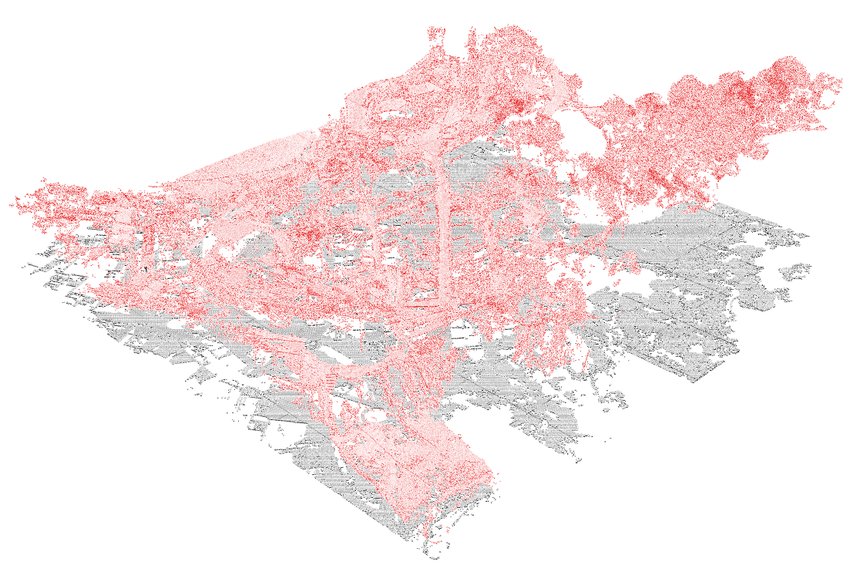
\includegraphics[width=0.3\textwidth]{png/nuvolPunts.png}}
    \caption{Exemple de núvol de punts en un espai tridimensional.}
    \label{fig:nuvolDePunts}
\end{figure}

En el context d’aquesta pràctica, les propietats que més ens interessen dels núvols de punts són:

\begin{itemize}
    \item \textbf{Distribució espacial}: en aquesta pràctica és uniforme, però en altres contextos podria seguir una distribució normal, exponencial, etc.
    \item \textbf{Densitat local}: determina com de propers poden estar els punts entre ells, fet que afecta el càlcul de distàncies mínimes.
    \item \textbf{Dimensionalitat}: treballam amb 2D, però els mateixos principis poden estendre’s a 3D o més dimensions, amb implicacions computacionals importants.
    \item \textbf{Ordenació}: per tal d’aplicar tècniques com el Divideix i Venceràs, cal ordenar prèviament els punts segons una coordenada (tipus sort per coordenada \(x\)).
\end{itemize}

La generació d’un núvol de punts és el punt de partida de la pràctica. A partir d’aquesta representació espacial:
\begin{itemize}
    \item Es calcula la distància entre parelles de punts, utilitzant mesures euclidianes.
    \item Es dissenyen algorismes per trobar el parell de punts més propers, optimitzant el temps de càlcul segons la mida del conjunt.
    \item Es visualitza la distribució espacial per verificar la correcció dels resultats.
\end{itemize}

Els núvols de punts proporcionen així una estructura de dades que és, alhora, simple i rica en potencial analític, sent un element central del problema resolt en aquesta pràctica.

\section{Entorn de Programació}

Per dur a terme el desenvolupament d’aquesta pràctica, s’ha fet ús d’un conjunt consolidat d’eines i tecnologies que han proporcionat un entorn robust, eficient i adaptable per a la implementació de l’algorisme basat en la tècnica de Divideix i Venceràs. A continuació es detallen les eines principals emprades:

\begin{itemize} 
    \item \textbf{Llenguatge de programació: Java} \ El projecte s’ha desenvolupat íntegrament amb Java, un llenguatge orientat a objectes conegut per la seva estabilitat, portabilitat i vasta col·lecció de llibreries estàndard. Java permet escriure codi clar i mantenible, a més d’oferir independència de plataforma mitjançant la màquina virtual (JVM), afavorint la portabilitat del projecte en diferents sistemes operatius.
    \item \textbf{Llibreries gràfiques: Swing i JavaFX} \\
    Per a la construcció de la interfície gràfica s’ha utilitzat la llibreria Swing, integrada dins del JDK. Aquesta llibreria proporciona els components necessaris per dissenyar interfícies gràfiques riques, amb una elevada capacitat de personalització i control dels esdeveniments gràfics. La seva estructura basada en el model MVC s’alinea bé amb l’arquitectura del projecte.

    Per a la construcció del visualitzador del gràfic en 3D s'ha emprat JavaFX. Aquesta llibreria proprorciona eines per a generar entorns tridimensionals i la interacció amb aquest. Gràcies a la integració Swing-JavaFX ha estat possible utilitzar aquesta llibreria
    
    \item \textbf{Entorn de desenvolupament: IntelliJ IDEA} \\
    IntelliJ IDEA ha estat l’IDE emprat per desenvolupar la pràctica. Aquesta eina ofereix funcionalitats avançades com autocompletat intel·ligent, anàlisi de codi en temps real, refactoritzacions guiades i integració amb eines externes com Git. 
    
    \item \textbf{Sistema de control de versions: GitHub} \\
    Per gestionar el codi font i controlar-ne l’evolució, s’ha utilitzat Git com a sistema de control de versions, amb GitHub com a repositori remot. 
\end{itemize}

L’elecció d’aquest conjunt d’eines ha permès garantir un desenvolupament estructurat i una gestió eficient del projecte, seguint bones pràctiques de disseny i facilitant la implementació de l’algorisme d’anàlisi de distància mínima sobre núvols de punts.


\section{Metodologia}

La implementació del model segueix una estructura modular basada en el patró \textit{Model-Vista-Controlador} (MVC). El model, en particular, es divideix en diversos paquets per a una organització òptima del codi, facilitant així la reutilització, manteniment i extensió de les diferents parts del sistema. A continuació, es descriuen les parts fonamentals del model, que inclouen les classes i els algorismes emprats per al càlcul de distàncies entre punts en un conjunt de dades generat aleatòriament.

\subsection{Paquet \texttt{model.calculs}}

Aquest paquet conté la classe abstracta \texttt{Calcul} i les seves implementacions concretes.

\begin{itemize} \item \textbf{Classe \texttt{Calcul}}: Aquesta classe abstracta serveix com a classe base per als diferents càlculs que es realitzen sobre el conjunt de punts. Defineix els atributs comuns per a totes les classes que hereten d'ella, com són la llista de punts (\texttt{punts}) i l'objecte \texttt{Dades}, que emmagatzema els resultats dels càlculs. Aquesta estructuració permet centralitzar la gestió de dades comunes a totes les implementacions concretes i simplificar l'extensió del sistema per afegir nous càlculs sense necessitat de duplicar el codi comú.

La classe \texttt{Calcul} implementa la interfície \texttt{Runnable}, la qual permet que els càlculs es realitzin en fils separats. Això facilita l'execució paral·lela dels càlculs i, per tant, millora el rendiment global de l'aplicació quan es treballa amb conjunts de punts grans.

Els càlculs concrets que es realitzen, com la recerca de la parella de punts més propera o la implementació de l'algorisme de \textit{Divideix i Venceràs}, es poden afegir fàcilment com a subclases que hereten de \texttt{Calcul}. A cada una d'elles se li passa la llista de punts i l'objecte \texttt{Dades}, el qual s'actualitza amb els resultats obtinguts després d'executar el mètode \texttt{run} que s'implementa en les subclases concretes. Així, \texttt{Calcul} no només proporciona una estructura bàsica i reutilitzable, sinó que també facilita la gestió de resultats i la seva presentació.

\begin{lstlisting}[language=java]
abstract class Calcul implements Runnable {

    protected final List<Punt> punts;
    protected Dades dades;

    public Calcul(List<Punt> punts) {
        this.dades = Main.instance.getDades();
        this.punts = new ArrayList<>(dades.getPunts());
    }
}
\end{lstlisting}

\end{itemize}

\begin{itemize} \item \textbf{Classe \texttt{ParellaPropera\_fb}}: Aquesta classe concreta implementa el càlcul de la parella de punts més propera mitjançant una aproximació de força bruta. El mètode \texttt{run} recorre totes les parelles de punts, calcula la distància entre elles i actualitza el resultat quan es troba una distància menor. Els resultats es guarden a l'objecte \texttt{Dades} per a la seva posterior visualització i anàlisi. A continuació, es mostra un fragment del codi de la classe \texttt{ParellaPropera\_fb}:
\\\\
\begin{lstlisting}[language=java]
public void run() {
    double min = Double.MAX_VALUE;
    Punt p1 = null, p2 = null;
    long t = System.nanoTime();
    for (int i = 0; i < punts.size(); i++) {
        for (int j = i + 1; j < punts.size(); j++) {
            double d = punts.get(i).distancia(punts.get(j));
                if (d < min) {
                    min = d;
                    p1 = punts.get(i);
                    p2 = punts.get(j);
                }
        }
    }
    t = System.nanoTime() - t;
    dades.addForcaBruta(p1, p2, min, t, "min");
}
\end{lstlisting}

\end{itemize}

\begin{itemize}
\item \textbf{Classe \texttt{ParellaPropera\_dv}}: Aquesta altra classe implementa una estratègia eficient per al càlcul de la parella de punts més propera mitjançant el paradigma de Divideix i Venceràs. El mètode \texttt{run} comença ordenant els punts per la seva coordenada X i crida el mètode recursiu \texttt{divideix}, que divideix l'espai de punts en dues meitats. 

La recursivitat s'atura quan el nombre de punts és petit (menor o igual a tres), cas en què es recorre a una solució de força bruta. Per a cada pas recursiu, es calcula la millor parella a l'esquerra i a la dreta i es determina la millor distància mínima global. A continuació, s'examina una franja vertical centrada en la mediana per detectar possibles parelles òptimes amb punts propers a la frontera. Aquesta franja es construeix amb punts que es troben a una distància menor que la mínima trobada respecte al pla vertical mitjà.

\begin{figure}[htbp]
    \centerline{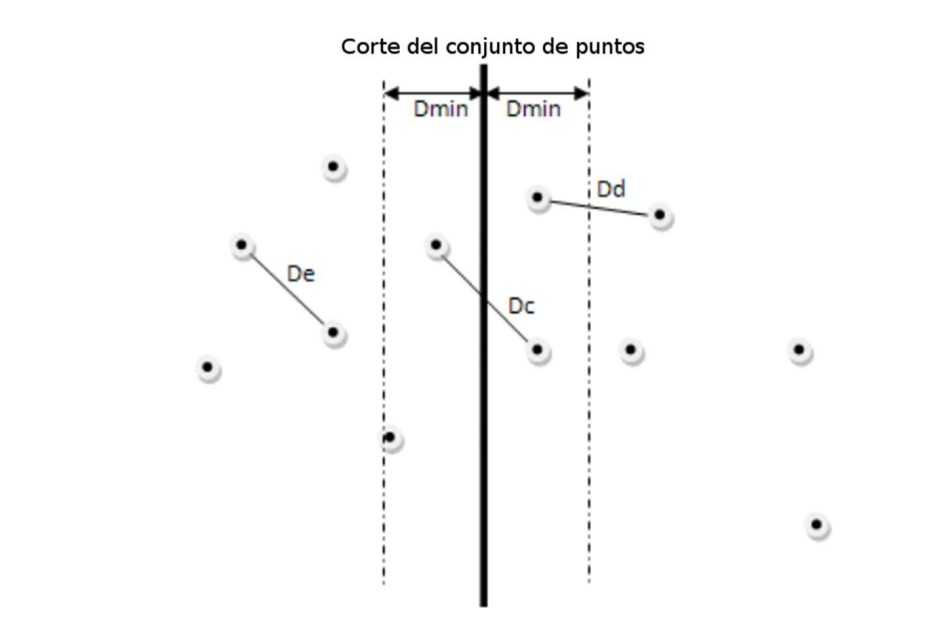
\includegraphics[width=0.3\textwidth]{docs/png/distMin.jpg}}
    \caption{Franja vertical centrada en la mediana per trobar parelles òptimes.}
    \label{fig:distMin}
\end{figure}

Els punts dins la franja s'ordenen per la coordenada Y, i s'estudien totes les possibles combinacions que poden millorar la distància mínima actual, respectant les restriccions geomètriques per reduir el nombre de comparacions. El tractament contempla tant punts en 2D com en 3D, segons la configuració establerta amb el paràmetre \texttt{TipoPunt}.
\end{itemize}

\begin{itemize}
\item \textbf{Classe \texttt{ParellaPropera\_kd}}: 
Aquesta classe calcula la distància mínima entre dos punts d’un núvol de punts, aprofitant l’eficiència que ofereix la implementació d’un arbre k-d.

En primer lloc, es construeix l’arbre k-d, on cada node conté un punt del conjunt original i pot tenir, com a màxim, dos fills: un amb una coordenada inferior i un altre amb una coordenada superior segons un eix determinat. A cada nivell de l’arbre es selecciona un eix de comparació alternant (per exemple, X, Y, Z en 3D) per dividir els punts de forma equilibrada. Aquesta estructura jeràrquica permet optimitzar la cerca de punts propers, reduint significativament el nombre de comparacions necessàries.

Un cop construït l’arbre, per a cada punt \( p \), es realitza una cerca del seu veí més proper. Al final del procés, es retorna la distància mínima trobada entre qualsevol parella de punts.

El cost computacional global és de \( O(n \log n) \). La construcció de l’arbre es realitza en \( O(n \log n) \), mentre que la cerca del punt més proper per a cada element del conjunt, tot i recórrer tots els punts una vegada (\( O(n) \)), es beneficia de cerques logarítmiques (\( O(\log n) \)) gràcies a l’estructura de l’arbre. Per tant, el cost total de l’algorisme es manté dins de l’ordre \( O(n \log n) \).

\end{itemize}

\begin{itemize}
\item \textbf{Classe \texttt{ParellaMaximaUniforme}}: Aquesta classe s'encarrega de calcular la parella de punts més llunyana dins un conjunt generat uniformement. Per tal de fer-ho de manera eficient, s'aprofita el fet que, en una distribució uniforme, els punts més allunyats es troben habitualment als extrems del conjunt. 

L'estratègia seguida consisteix a detectar aquests punts extrems mitjançant combinacions lineals de les seves coordenades (com per exemple $x + y$, $x - y$, $-x + y$, $-x - y$). Aquestes combinacions permeten localitzar els punts situats a les quatre cantonades del conjunt convex. 

Finalment, es comparen les dues diagonals formades per aquests punts per determinar quina és la parella amb la distància màxima. Aquesta aproximació redueix dràsticament el nombre de comparacions respecte a una estratègia de força bruta.
\end{itemize}

\begin{itemize}
\item \textbf{Classe \texttt{ParellaMaxima\_CH}}: Aquesta classe s'encarrega de calcular la parella de punts més llunyana. Per a aconseguir-ho, es crea la figura convexa que agrupa tots els punts del núvol, polígon o poliedre depenent de la dimensió del conjunt. Finalment amb els punts vèrtex de la figura resultant es fa una cerca amb força bruta, que encara sigui \(O(n^2)\), es fa sobre un conjunt molt reduït respecte l'original, per tant la complexitat global general es \(O(nlog(n))\).

Aquesta classe en concret te la implementació del algorisme de "Graham scan" \cite{GrahamScan} per a generar el polígon convex dels punts en 2D. Aquest algorisme genera el polígon en complexitat \(O(nlog(n))\) al ordenar els punts amb el angle respecte a un punt inicial i operant seqüencialment amb una pila.

Per al 3D s'utilitza una altra tècnica a \texttt{ParellaMaxima\_QH}.

\end{itemize}

\begin{itemize}
\item \textbf{Classe \texttt{ParellaMaxima\_QH}}: 
Aquesta classe en concret te la implementació del algorisme de "Quick Hull 3D" \cite{quickhull} per a generar el polígon convex dels punts en ·D. Aquest algorisme genera el polígon en complexitat \(O(nlog(n))\) al generar de forma iterativa les diferents cares del poliedre, descartant els punts que queden dins la figura.

Degut a la complexitat d'aquest algorisme, i al tractar-se d'una part extra per al càlcul de distància màxima, s'ha optat per adaptar un codi fer per John E. Lloyd \cite{John}, amb una llicencia que permet el seu ús, modificació i distribució sempre que s'acrediti a l'autor original.

\end{itemize}



\subsection{Paquet \texttt{model.generadors}}

El paquet \texttt{model.generadors} conté les classes encarregades de generar els conjunts de punts segons diferents distribucions. La classe \texttt{Generador} és abstracta i defineix la interfície general per a tots els generadors de punts, mentre que les seves subclasses implementen lògiques específiques per a la generació de punts segons diferents distribucions.

\begin{itemize} \item \textbf{Classe \texttt{Generador}}: Aquesta classe abstracta defineix les propietats comunes com el nombre de punts (\texttt{n}) i els límits de la distribució (\texttt{min} i \texttt{max}). La seva principal responsabilitat és definir el mètode abstracte \texttt{genera}, que serà implementat per les subclases per generar els punts.

\begin{lstlisting}[language=java]
public abstract class Generador {
    protected int n;
    protected int min;
    protected int max;

    public Generador(int n, int min, int max) {
        this.n = n;
        this.min = min;
        this.max = max;
    }

    public abstract List<Punt> genera();
}


\end{lstlisting}

\item \textbf{Classe \texttt{GeneradorUniforme}}: Aquesta classe és una implementació concreta de \texttt{Generador} que genera punts aleatoris dins d'un interval [\texttt{min}, \texttt{max}] per a cada coordenada. La generació de punts es realitza mitjançant la classe \texttt{Random}, i els punts generats es representen, per exemple, com a objectes de la classe \texttt{Punt2D}, una subclasse de \texttt{Punt}. A continuació es mostra l'algorisme per generar els punts en un espai bidimensional de forma uniforme:

\begin{lstlisting}[language=java]
public List<Punt> genera2() {
    List<Punt> punts = new ArrayList<>();
    for (int i = 0; i < n; i++) {
        int x = rand.nextInt(max - min + 1) + min;
        int y = rand.nextInt(max - min + 1) + min;
        punts.add(new Punt2D(x, y));
    }
    return punts;
}
\end{lstlisting}


\end{itemize}

\begin{itemize}
\item \textbf{Altres generadors implementats}: A més del generador uniforme, s'han implementat dues variants més per obtenir distribucions alternatives de punts: el generador gaussià i el generador exponencial. Ambdós generadors hereten de la classe \texttt{Generador} i redefineixen els mètodes per generar coordenades amb diferents distribucions estadístiques.

\begin{itemize}
    \item \textbf{Generador Gaussià}: Utilitza la funció \texttt{rand.nextGaussian()} per generar valors distribuïts normalment amb mitjana i desviació estàndard triades aleatòriament al principi de l'execució del programa.
    Això permet simular núvols de punts concentrats entorn a una regió central, útils per a anàlisi de rendiment sota distribucions no uniformes.

    \item \textbf{Generador Exponencial}: Utilitza la fórmula de la transformada inversa per obtenir valors segons una distribució exponencial amb paràmetre \(\lambda\).
    Aquesta distribució és útil per simular casos on hi ha gran concentració de punts en una zona i dispersió progressiva en la resta.
\end{itemize}
\end{itemize}

\begin{itemize}
\item \textbf{Classe \texttt{KdArbre}}: Aquesta classe implementa un \textit{kd-tree} per a punts de k-dimensions. La seva finalitat és organitzar eficientment els punts per tal d'optimitzar consultes com la cerca de la parella de punts més propera. El kd-tree s'utilitza com a alternativa a altres estructures com ara els arbres binaris o llistes ordenades, ja que ofereix millor rendiment en consultes espacials locals.

\begin{itemize}
    \item \textbf{Estructura de dades}: Cada node del kd-tree conté un punt kD i referències als seus fills esquerre i dret. A més, la separació entre els nodes es fa alternant les dimensions \(x\) i \(y\) a cada nivell de profunditat, permetent una partició eficient de l'espai.

    \item \textbf{Mètode \texttt{inserir(Punt2D p)}}: Aquest mètode insereix un nou punt al kd-tree seguint el criteri de divisió per coordenades alternades. 

    \item \textbf{Mètode \texttt{cercarPropera(Punt2D p)}}: Aquest mètode retorna el punt més proper al punt \(p\) dins del kd-tree. Es basa en una recerca recursiva que compara distàncies i aprofita l'estructura del kd-tree per descartar branques innecessàries (pruning).
\end{itemize}
\end{itemize}


\subsection{Paquet \texttt{model.punts}}

Aquest paquet defineix la classe \texttt{Punt}, que és una classe abstracta per representar punts en l'espai, així com les seves subclasses concretes com \texttt{Punt2D}. La classe \texttt{Punt} defineix el mètode abstracte \texttt{distancia}, que es reimplementa a les subclasses per calcular la distància entre dos punts.

\begin{itemize} \item \textbf{Classe \texttt{Punt}}: La classe \texttt{Punt} és abstracta i declara el mètode \texttt{distancia}, que serà implementat per les subclasses per calcular la distància entre punts de diferents dimensions.

\item \textbf{Classe \texttt{Punt2D}}: Aquesta classe concreta implementa el mètode \texttt{distancia} per calcular la distància euclidiana entre dos punts en un espai 2D. La fórmula utilitzada és la següent:

\[
\text{distància} = \sqrt{(x_1 - x_2)^2 + (y_1 - y_2)^2}
\]

A continuació es mostra el codi de la classe \texttt{Punt2D}:

\begin{lstlisting}[language=java]
public class Punt2D extends Punt {
    public final int x, y;

    public Punt2D(int x, int y) {
        this.x = x;
        this.y = y;
    }

    public double distancia(Punt punt2) {
        Punt2D altre = (Punt2D) punt2;
        double dx = this.x - altre.x;
        double dy = this.y - altre.y;
        return Math.sqrt(dx * dx + dy * dy);
    }
}
\end{lstlisting}


\end{itemize}

\subsection{Classe \texttt{Dades}}

\begin{itemize} \item \textbf{Classe \texttt{Dades}}: Aquesta classe és responsable de gestionar i emmagatzemar els resultats obtinguts dels càlculs realitzats, separant-los dins un Map segons el tipus de calcul utilitzat (Força Bruta, DiV, etc). D'aquesta forma es té d'una forma compacta i eficient els diferents resultats per a poder visualitzarlos posteriorment.

La classe \texttt{Dades} disposa de mètodes per afegir resultats al mapa, així com per accedir a aquests resultats. Quan es calcula una parella de punts i la seva distància, es crida al mètode \texttt{afegeixResultat}. Aquests mètodes creen un objecte de la classe interna \texttt{Resultat}, el qual emmagatzema els punts calculats, la distància entre ells, el temps que ha durat el càlcul i el tipus d'algorisme utilitzat. Els resultats es mantenen en aquests mapa per a poder ser recuperats posteriorment per mostrar-los a l'usuari o per realitzar anàlisis addicionals.

La definició de la classe \texttt{Dades} permet centralitzar la gestió dels resultats, simplificant el codi i evitant la necessitat de passar els resultats de manera manual entre diferents parts de l'aplicació. A més, la classe interna \texttt{Resultat} encapsula la informació rellevant de cada càlcul, millorant l'organització del codi i la seva llegibilitat.


\begin{lstlisting}[language=java]
public class Dades {
    private final TreeMap<TipusCalcul, List<Resultat>> resultats;

    public Dades() {
        this.resultats = new TreeMap<>();
    }

    public void afegeixResultat(int n, Punt p1, Punt p2, double distancia, long tempsNano, TipusCalcul calcul)
}
\end{lstlisting}

El disseny de la classe permet gestionar de manera eficient els resultats obtinguts en els càlculs, alhora que facilita la seva extensibilitat per afegir nous mètodes o llistes en el futur, si calgués ampliar les funcionalitats de l'aplicació.

\end{itemize}

\subsection{Controlador}

\begin{itemize}
\item \textbf{Classe \texttt{Main} (Controlador)}: La classe \texttt{Main} actua com a controlador central del sistema, gestionant la comunicació entre la interfície gràfica (\texttt{Finestra}), les dades (\texttt{Dades}), i les diferents funcionalitats del model (generadors de punts i algorismes de càlcul). Aquesta classe implementa la interfície \texttt{Comunicar}, la qual defineix un mecanisme unificat per rebre instruccions des de la vista.

\begin{itemize}
    \item \textbf{Inici del sistema}: L'execució del programa comença amb el mètode \texttt{main}, el qual crea una instància del controlador i crida el mètode \texttt{init}. En aquest mètode s’instancien les dades i es llença la creació de la vista mitjançant \texttt{SwingUtilities.invokeLater}, assegurant que la GUI es construeixi al fil d'execució d'AWT.

    A més, per simplesa de codi, Main és un Singleton \cite{singleton}, que permet l'accés a la instancia des de les altres classes

    \begin{lstlisting}[language=java]
    public static void main(String[] args) {
        (new Main()).init();
    }

    private void init() {
        instance = this;
        dades = new Dades();
        punts = new ArrayList<>();
        processos = new ArrayList<>();
        SwingUtilities.invokeLater(() -> finestra = new Finestra());
    }
    \end{lstlisting}

    \item \textbf{Comunicació amb la vista}: La classe rep missatges de la GUI mitjançant el mètode \texttt{comunicar(String msg)}, que actua com un gestor de comandes. Aquest mètode analitza el missatge rebut i executa la funcionalitat corresponent, com generar punts, calcular distàncies o esborrar dades. Aquesta arquitectura basada en missatges permet una separació clara entre la vista i la lògica.

    \item \textbf{Generació de punts}: Quan es rep un missatge del tipus \texttt{"generar:\dots"}, el controlador identifica el tipus de punt, la distribució i els paràmetres necessaris, i invoca dinàmicament el constructor del generador adequat mitjançant reflexió. A més, si el nombre de punts és suficientment gran s'invoca la versió concurrent per a la generació de punts. Un cop generats, els punts s’emmagatzemen en l’objecte \texttt{Dades} i s’actualitza la vista.

    \begin{lstlisting}[language=java]
    generarPunts(GENERADORS.get(distribucio), tp, params);
    finestra.comunicar("dibuixPunts");
    \end{lstlisting}

    \item \textbf{Execució d'algorismes}: Per iniciar un càlcul de distàncies, el controlador rep un missatge \texttt{"calcular:\dots"} i instància el corresponent algorisme implementat a la jerarquia \texttt{Calcul}. L’execució es realitza en un fil separat mitjançant un \texttt{ExecutorService}, evitant bloquejos a la GUI. Després del càlcul, es comunica la vista perquè representi els resultats.
    
    Addicionalment, s’ha implementat l’execució paral·lela a nivell intern en alguns algorismes, com ara els de força bruta i els basats en arbres kd. Atès que el càlcul final de la distància mínima o màxima implica comparar cada punt amb la resta —és a dir, realitzar comparacions entre n i (n-1) punts per determinar la millor opció—, s'han llançat fils concurrents per processar múltiples valors de n simultàniament.

Aquesta concurrència s’integra dins el mètode run(), mitjançant el següent fragment de codi, sent calc2 la versió amb concurrència.     
    \begin{lstlisting}[language=java]
    res = Main.instance.isModeConcurrentOn()?  calc2((ArrayList<Punt>) punts):   calc((ArrayList<Punt>) punts);
    \end{lstlisting}

     

    \item \textbf{Gestió de processos concurrents}: Tots els processos de càlcul implementen la interfície \texttt{Comunicar}, cosa que permet que el controlador els pugui aturar si es rep la comanda \texttt{"aturar"}. Això garanteix el control sobre l'execució en paral·lel i evita càlculs simultanis no desitjats.

    \begin{lstlisting}[language=java]
    for (Comunicar proces : processos) {
        proces.comunicar("aturar");
    }
    processos.clear();
    \end{lstlisting}

    \item \textbf{Propòsit de la classe \texttt{Dades}}: Aquesta classe serveix com a magatzem compartit de la informació generada i dels resultats dels càlculs. El controlador l’utilitza per accedir i modificar els punts i els resultats sense haver de passar per la vista ni per cap classe específica del model.

    \item \textbf{Gestió extensible de generadors i algorismes}: El controlador fa ús de dos \texttt{Map} per relacionar cadenes literals amb les classes concretes de generadors i algorismes. Aquesta estructura permet ampliar fàcilment el sistema afegint nous tipus de generadors o estratègies de càlcul.

    \begin{lstlisting}[language=java]
    private static final Map<String, Class<? extends Generador>> GENERADORS = Map.of(
        "Uniforme", GeneradorUniforme.class,
        "Gaussiana", GeneradorGaussia.class,
        "Exponencial", GeneradorExponencial.class
    );
    \end{lstlisting}
\end{itemize}
\end{itemize}

\subsection{Vista}

La vista del projecte s'encarrega de representar gràficament la informació generada i calculada pel sistema. Aquesta es construeix seguint un enfocament modular i adaptable, que permet visualitzar tant representacions bidimensionals com tridimensionals del conjunt de punts i dels resultats del càlcul de distàncies.

\subsubsection*{Estructures principals de la vista}

La vista està formada per diversos components, entre els quals destaquen:

\begin{itemize}
    \item \textbf{\texttt{Finestra}}: És la classe principal de la vista, que hereta de \texttt{JFrame}. Aquesta defineix i organitza l'estructura gràfica de l'aplicació. Incorpora un panell de botons per a la interacció de l'usuari (generar punts, calcular distància, esborrar, etc.) i un panell central on es representen els eixos.
    
    \item \textbf{\texttt{Eixos2D}}: Classe encarregada de la visualització en dues dimensions. Hereta de \texttt{JPanel} i fa ús de l'API gràfica de \texttt{Swing}. Implementa els mètodes \texttt{paintComponent}, \texttt{pintarPunts} i \texttt{pintarDistancia} per renderitzar els punts i les distàncies calculades en el pla.
    
    \item \textbf{\texttt{Eixos3D}}: Aquesta classe proporciona la representació en tres dimensions utilitzant \texttt{JavaFX}. Hereta de \texttt{JFXPanel} i incorpora elements com \texttt{Camera}, \texttt{Group} i transformacions com rotacions i translacions per a permetre la navegació i observació del núvol de punts 3D d'una manera intuïtiva i responsiva.
    
    \item \textbf {\texttt{Enums : Dimensio i Distribucio}}: Serveixen per representar, respectivament, la dimensió dels punts (2D o 3D) i el tipus de distribució estadística emprada per a generar els punts (Uniforme, Gaussiana o Exponencial).

    \item\textbf{ \texttt{FinestraTempsExec}}:
    Extendeix d'un \texttt{JFrame} i serveix per visualitzar els temps d'exeucució dels algorismes per al càlcul de la distància propera.
    \item \textbf{\texttt{EixosTempsExec}}: Classe d'eixos de la gràfica pintada a la finestra \texttt{FinestraTempsExec}.
    
\end{itemize}

\subsubsection*{Funcionament i integració}

La classe \texttt{Finestra} actua com a punt d'entrada i gestió de tota la vista. Aquesta es registra com a entitat comunicadora mitjançant la interfície \texttt{Comunicar}, i rep missatges del controlador per modificar l'estat gràfic de la interfície.

Un fragment rellevant del constructor de \texttt{Finestra} mostra com s'inicialitzen els dos tipus d'eixos i s'insereixen al panell central:

\begin{itemize}
    \begin{lstlisting}[language=java]
    eixos = new Comunicar[]{new Eixos2D(), new Eixos3D()};
    currentEixos = eixos[0];
    
    cardLayout = new CardLayout();
    eixosPanel = new JPanel(cardLayout);
    
    eixosPanel.add((Component) eixos[0], Dimensio.D2.getEtiqueta());
    eixosPanel.add((Component) eixos[1], Dimensio.D3.getEtiqueta());
    this.add(eixosPanel, BorderLayout.CENTER);
    \end{lstlisting}
    
\end{itemize}


L'ús de \texttt{CardLayout} permet alternar de manera dinàmica entre la visualització 2D i la 3D segons la dimensió dels punts generats. L'objecte \texttt{currentEixos} manté una referència al component actual actiu, al qual es poden enviar missatges per actualitzar la representació.

Tots dos components gràfics \texttt{Eixos2D} i \texttt{Eixos3D} accedeixen a la informació necessària a través de l'objecte \texttt{Dades}, gestionat per la classe principal \texttt{Main}. Aquesta connexió garanteix una separació clara entre el model i la vista, seguint l'estil arquitectònic MVC.

\subsubsection*{Exemple visual}

A la figura següent es pot observar un exemple de la vista durant una execució del programa, mostrant punts generats.

\begin{figure}[htbp]
    \centerline{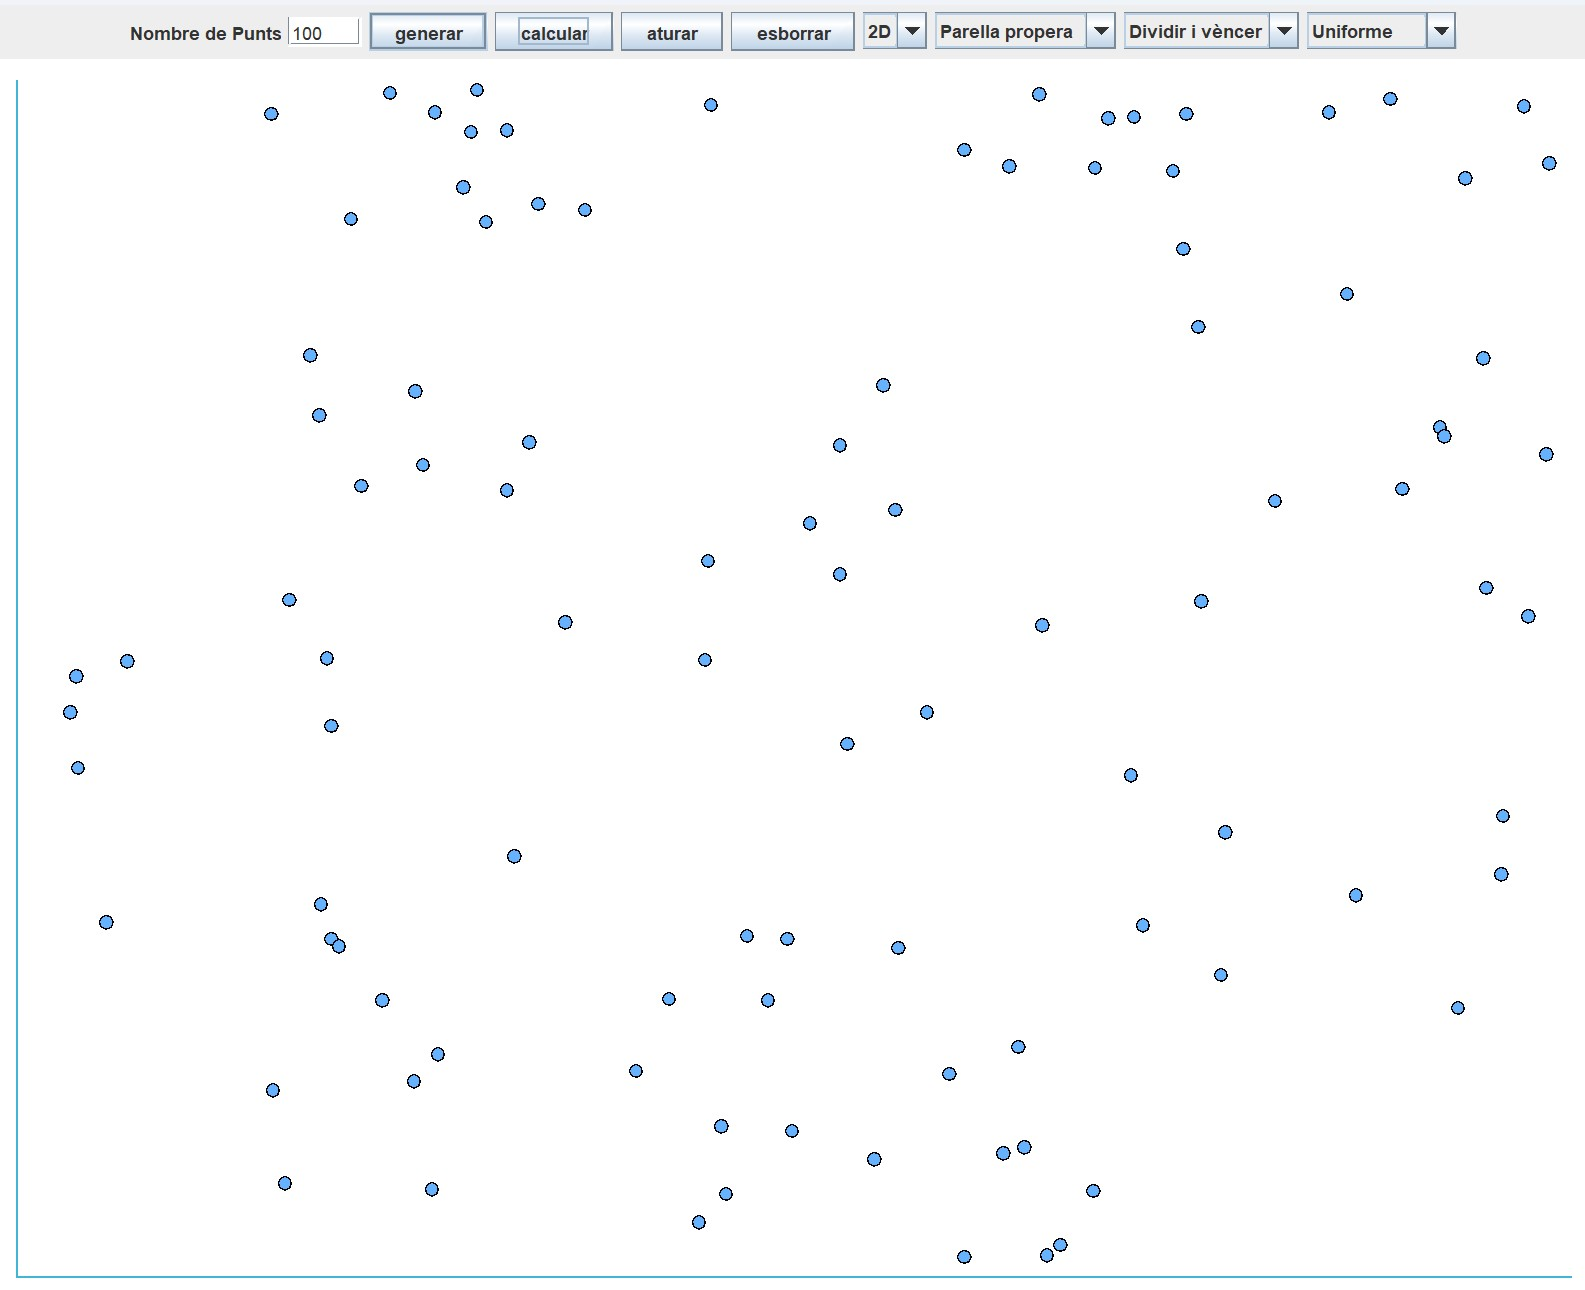
\includegraphics[width=0.45\textwidth]{docs/png/exempleVista.jpg}}
    \caption{Interfície gràfica de l'aplicació mostrant un núvol de punts en dues dimensions.}
    \label{fig:nuvol2D}
\end{figure}

\begin{figure}[htbp]
    \centerline{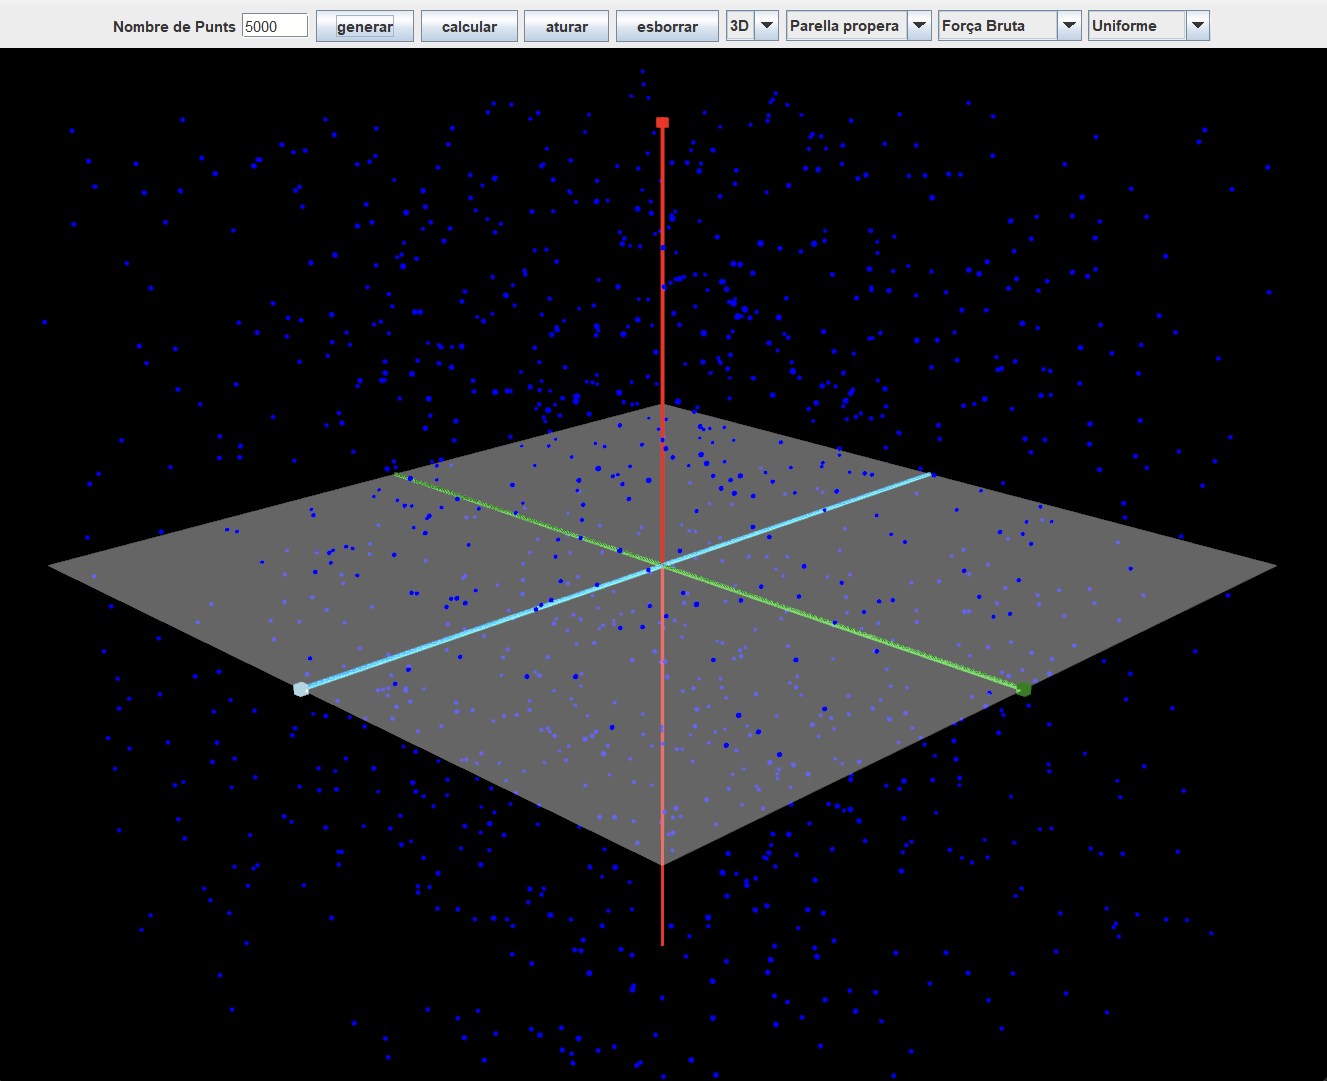
\includegraphics[width=0.45\textwidth]{docs/png/nuvolPunts3D.png}}
    \caption{Interfície gràfica de l'aplicació mostrant un núvol de punts en tres dimensions.}
    \label{fig:nuvol3D}
\end{figure}

\begin{figure}[htbp]
    \centerline{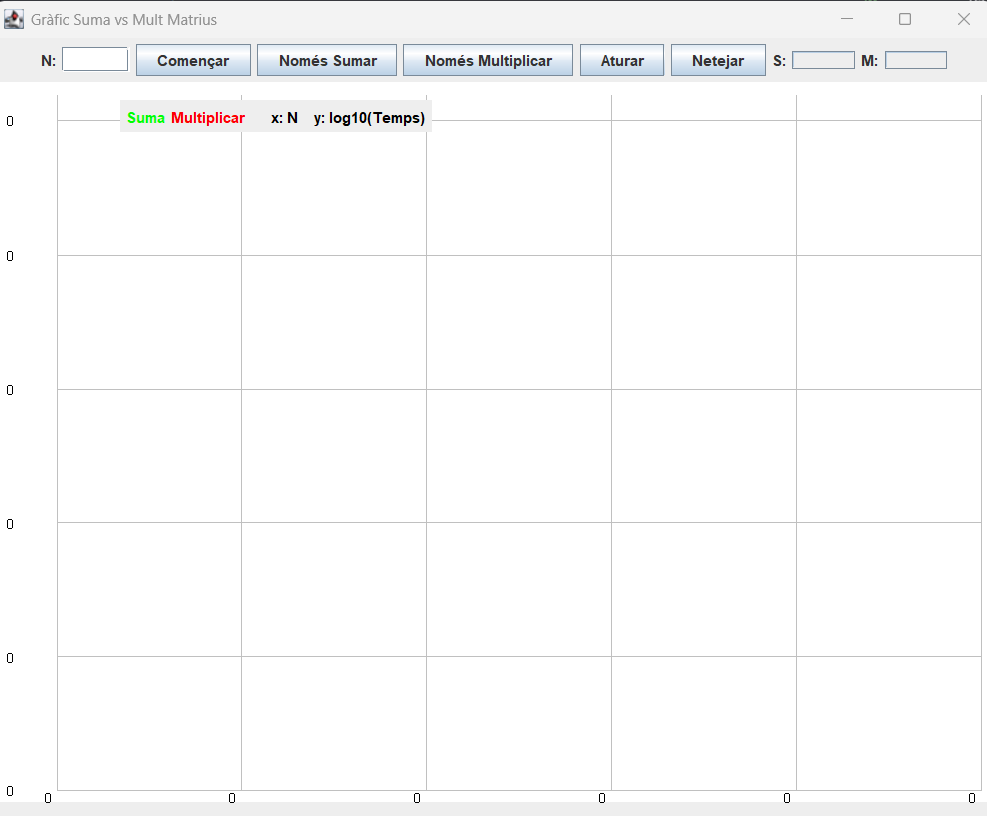
\includegraphics[width=0.45\textwidth]{docs/png/grafica.png}}
    \caption{Gràfica dels temps d'execució dels algorismes de càlcul de distàncies properes.}
    \label{fig:nuvol3D}
\end{figure}
\section{Arquitectura del Programa}

L’aplicació segueix una arquitectura basada en el patró Model-Vista-Controlador (MVC), que separa clarament la lògica de negoci, la interfície gràfica i el flux de control. Aquest enfocament facilita tant la mantenibilitat del codi com la seva extensibilitat futura.

El \textbf{model} encapsula les estructures de dades i la lògica algorísmica associada al càlcul de distàncies entre punts, incloent la generació de punts en dues i tres dimensions amb diferents distribucions, així com les estratègies per determinar les parelles més properes i més llunyanes.

La \textbf{vista} proporciona una representació gràfica intuïtiva del núvol de punts i els resultats, i es troba desacoblada del model. Permet commutar entre representacions 2D (\texttt{Swing}) i 3D (\texttt{JavaFX}) mitjançant una arquitectura flexible basada en \texttt{CardLayout}.

El \textbf{controlador}, integrat principalment a la classe \texttt{Main}, gestiona el flux d’execució i la comunicació entre el model i la vista. La comunicació entre components es basa en una interfície comuna (\texttt{Comunicar}), que garanteix la modularitat i redueix la dependència entre mòduls.

Aquesta arquitectura modular facilita l’evolució del sistema, per exemple permetent incorporar noves estratègies de càlcul o nous tipus de visualització sense afectar els altres components.




\section{Resultats i Comparació}

 En aquesta secció analitzarem l'eficiència dels algorismes implementats per al càlcul de la distància mínima i màxima, diferenciant-los segons la dimensió de l'espai (2D i 3D). Per avaluar-ne el rendiment, hem executat cadascun dels algorismes amb diferents quantitats de punts i hem mesurat el temps d'execució necessari per a completar el càlcul.

Els resultats obtinguts es recullen en les taules següents, on es mostra com varia el temps d'execució en funció del nombre de punts. Cal assenyalar que totes les proves s'han realitzat emprant una distribució uniforme de punts per garantir la comparabilitat dels resultats. 

\begin{table}[H]
    \centering
    \begin{tabular}{|c|c|c|c| }
        \hline
        \textbf{N} & \textbf{Força Bruta} & \textbf{D i C} & \textbf{Arbre-K}  \\
        \hline
         100    & 518200 &    1536000 &  3274100 \\
         1000  &  1474400 & 	22213000 &	6900700     \\
         10000  &   8510500&	104313000	&21987100  \\
         100000  & 18912300 &	207167600 &	33500900  \\
         1000000  & 128012500 &	4176033700 &563527000 \\
      
        \hline
    \end{tabular}
    \vspace{3mm}
    \caption{Temps d'execució del càlcul de la distància mínima en 2D en nanosegons}
    \label{tab:complexitat}
\end{table}

\begin{table}[H]
    \centering
    \begin{tabular}{|c|c|c|c| }
        \hline
        \textbf{N} & \textbf{Força Bruta} & \textbf{D i C} & \textbf{Arbre-K}  \\
        \hline
         100    & 1207800&	3230500	&3006600 \\
         1000  & 10696700&	11950000	&7165600     \\
         10000  &  220977000	&39791800	&15186000 \\
         100000  & 13600600&	35392600&	33121300  \\
         1000000  & 21832400&	634317800	&278436300 \\
      
        \hline
    \end{tabular}
    \vspace{3mm}
    \caption{Temps d'execució del càlcul de la distància mínima en 3D en nanosegons}
    \label{tab:complexitat}
\end{table}

\begin{table}[H]
    \centering
    \begin{tabular}{|c|c|c|c| }
        \hline
        \textbf{N} & \textbf{Força Bruta} & \textbf{D i C} & \textbf{Arbre-K}  \\
        \hline
         100    & 333100	&43700	&491600 \\
         1000  &  3921800 &	104400	&4331200    \\
         10000  & 166943400&	879800&	24945900  \\
         100000  & 4044000	&911500	&41775900  \\
         1000000  & 62995800&	16740500&	336016600 \\
      
        \hline
    \end{tabular}
    \vspace{3mm}
    \caption{Temps d'execució del càlcul de la distància màxima en 2D en nanosegons}
    \label{tab:complexitat}
\end{table}

 \begin{table}[H]
    \centering
    \begin{tabular}{|c|c|c|c| }
        \hline
        \textbf{N} & \textbf{Força Bruta} & \textbf{D i C} & \textbf{Arbre-K}  \\
        \hline
         100    &411000&	1440000	& 3822700 \\
         1000  &  10865700 &	1095500&	3494300    \\
         10000  &   152053200 &	2942000	&18271000 \\
         100000  & 11195200&	5460500	&47172700  \\
         1000000  & 60304200 &	10449100&	368713700 \\
      
        \hline
    \end{tabular}
    \vspace{3mm}
    \caption{Temps d'execució del càlcul de la distància màxima en 3D en nanosegons}
    \label{tab:complexitat}
\end{table}


\begin{figure}[H]
    \centerline{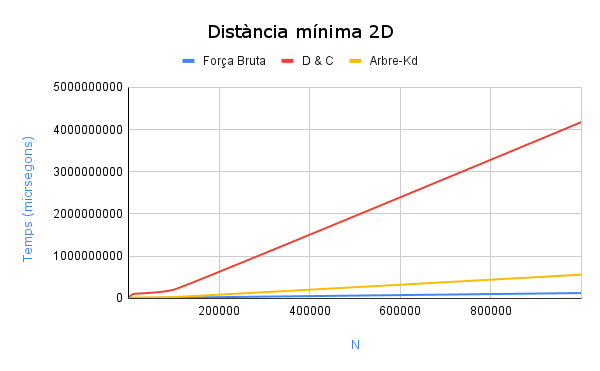
\includegraphics[width=0.45\textwidth]{docs/png/Distància mínima 2D.png}}
    \caption{Distància mínima (parella propera) en 2D.}
    \label{fig:distMin}
\end{figure}

\begin{figure}[h]
    \centerline{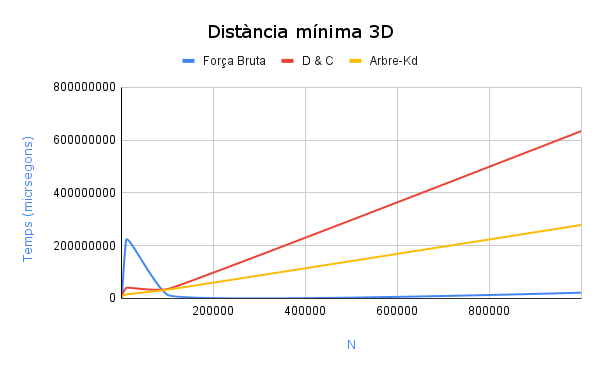
\includegraphics[width=0.45\textwidth]{docs/png/Distància mínima 3D.png}}
    \caption{Distància mínima (parella propera) en 3D.}
    \label{fig:distMin}
\end{figure}


\begin{figure}[H]
    \centerline{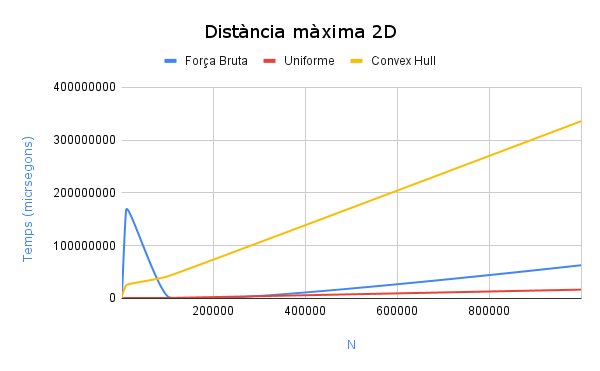
\includegraphics[width=0.45\textwidth]{docs/png/Distància màxima 2D.png}}
    \caption{Distància màxima (parella llunyana) en 2D.}
    \label{fig:distMin}
\end{figure}

\begin{figure}[h]
    \centerline{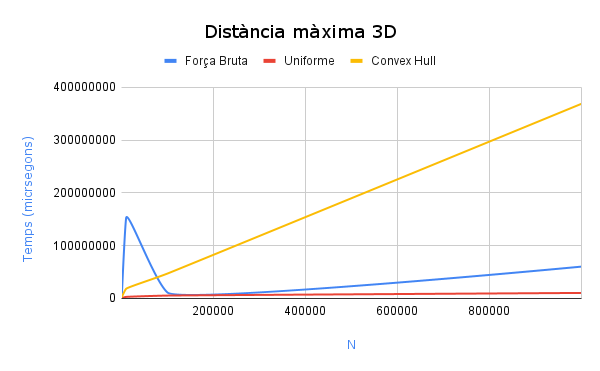
\includegraphics[width=0.45\textwidth]{docs/png/Distància màxima 3D.png}}
    \caption{Distància màxima (parella llunyana) en 3D.}
    \label{fig:distMin}
\end{figure}

\section*{Anàlisi dels resultats experimentals}

A continuació analitzarem les gràfiques generades per als càlculs de parelles de punts en funció de la seva distància, tant per a l'espai bidimensional com tridimensional.

\subsection*{Càlcul de la distància mínima (parelles properes)}

\paragraph{Espai 2D.}
En el cas d'un espai bidimensional, s'ha observat que l'algorisme basat en l'estratègia de \textit{Dividir i Vèncer} és el més costós computacionalment. Això es feu a que, per conjunt de punts de mida moderada, la sobrecàrrega associada amb:
\begin{itemize}
    \item La divisió recursiva del conjunt de punts,
    \item La combinació dels resultats parcials,
    \item L'ordenació final de la llista de punts,
\end{itemize}
compensa els avantatges teòrics que ofereix aquesta estratègia (complexitat \(O(n\log n)\) en el cas asimptòtic). En canvi, tot i que la \textbf{força bruta} té una complexitat de \(O(n^2)\), la seva simplicitat permet obtenir un rendiment superior per a nombres de punts relativament baixos. Així mateix, els algorismes basats en \textbf{arbres kd} mostren resultats molt satisfactoris, semblants als de la força bruta, indicant que també són molt efectius per a conjunts de mida moderada.

\paragraph{Espai 3D.}
En l'espai tridimensional es nota un comportament similar. L'algorisme de força bruta resulta, en termes pràctics, és el més eficient per a conjunts de dades petits o moderats. No obstant això, s'observa que a mesura que el nombre de punts s'incrementa (per exemple, amb \(N = 10\,000\)) es produeix un augment significatiu en el temps d'execució, el que s'anomena punt d'inflexió. Aquest comportament s'atribueix, en part, a la gestió de recursos i l'estabilització interna de la màquina virtual (JVM) davant d'un augment en la càrrega de treball. Algorismes com ara \textit{Dividir i Vèncer} i els basats en \textbf{Arbre-Kd}, tot i tenir millor rendiment asimptòtic, presenten una sobrecàrrega en les operacions de divisió, combinació i ordenació, fent-los menys eficients en aquest rang.

\subsection*{Càlcul de la distància màxima}


Les gràfiques obtengudes mostren que, en ambdós espais (2D i 3D), l'algorisme basat en \textbf{Convex Hull} no resulta tan eficient com s'esperava. Tot i que teòricament té una complexitat de \(O(n\log n)\), les constants elevades associades a la construcció de l'envoltòria convexa afecten negativament el seu rendiment. En canvi, l'algorisme \textbf{Uniforme} ha mostrat millors resultats en termes de temps d'execució, arribant a ser fins i tot més eficient que la força bruta per a certs rangs del nombre de punts i sobretot en l'espai bidimensional.

\subsection*{Punt d'inflexió i estabilització}

En totes les gràfiques es pot identificar un \emph{punt d'inflexió}: és a dir, un punt en què, a mesura que augmenta el nombre de punts, hi ha un salt significatiu en el temps d'execució, i més endavant el temps tendeix a estabilitzar-se. Aquest comportament podria ser resultat de:
\begin{itemize}
    \item L'augment del nombre d'operacions (comparacions, ordenacions, etc.) necessàries per tractar conjunts més grans.
    \item Optimitzacions internes de la JVM, que redueixen la penalització temporal després d'un cert llindar.
\end{itemize}

\section*{Costos asimptòtics dels algorismes}

Per comprendre millor el comportament experimental, es resumeixen a continuació els costos asimptòtics (en notació Big-O) dels diferents algorismes:

\begin{table}[h]
    \centering
    \begin{tabular}{|l|l|}
        \hline
        \textbf{Algorisme} & \textbf{Cost Computacional} \\
        \hline
        Força Bruta         & \(O(n^2)\)       \\
        Dividir i Vèncer    & \(O(n\log n)\)   \\
        Arbre-Kd            & \(O(n\log n)\)   \\
        Uniforme-2D         & \(O(n)\)         \\
        Uniforme-3D         & \(O(n\log n)\)   \\
        Convex Hull         & \(O(n\log n)\)   \\
        \hline
    \end{tabular}
    \vspace{3mm}
    \caption{Costos d'execució dels algorismes per al càlcul de distàncies.}
    \label{tab:complexitat}
\end{table}

\bigskip

\noindent En resum, tot i que algorismes com \textit{Dividir i Vèncer} o els basats en \textbf{Arbre-Kd} presenten una complexitat asimptòtica millor que la força bruta, la seva implementació més complexa, i poc optimitzada en el nostre cas,  genera una sobrecàrrega que resulta en temps d'execució superiors per a conjunts de dades relativament petits o moderats. Aquesta comparativa entre complexitat teòrica i rendiment pràctic ens ajuda a decidir quin algorisme és més adient en funció del nombre de punts i la natura de la distribució de les dades.



\section{Conclusions}
En conclusió, aquesta pràctica ha requerit una dedicació considerable de temps per poder-la dur a terme. S’ha produït un cert desequilibri en el repartiment de la feina, ja que alguns membres de l’equip han hagut d’assumir les parts més complexes del projecte, una situació que es podria haver evitat amb una millor planificació i coordinació. A més, començar la pràctica amb només una setmana abans de la data límit d'entrega no ha estat l’escenari més òptim, i això ha afectat negativament tant l’organització com el rendiment global.

D’altra banda, per desenvolupar les funcionalitats opcionals ha estat necessari consultar materials addicionals, ja que alguns conceptes no eren del tot intuïtius. En el cas de la implementació dels arbres Kd, hem comptat amb el suport d’un article científic que explicava de forma clara tant el funcionament com la pseudo-codificació de l’algorisme. Pel que fa a la implementació en 3D i a l’algorisme del Convex Hull, aquestes s’han basat parcialment en codis font de referència trobats en recursos externs.

És important també recalcar que el warning que mostra JavaFX per consola al executar el programa es deu a que JavaFX va ser incorporat mitjançant el desenvolupament de la pràctica i no es va poder configurar correctament. (JavaFX vol ser un modul apart i no inclòs dins el principal). Igualment no hi ha hagut cap problema amb JavaFX, per tant es pot ignorar l'error.

I com a última reflexió, la implementació del paral·lelisme intern en els algorismes de generació de punts i en els càlculs de distàncies ha suposat una petita millora en el rendiment global del programa. No obstant això, atès que la concurrència comporta una càrrega addicional en l'organització dels fils d'execució i la seva sincronització, no sempre és la millor opció, especialment per a conjunts de punts petits. Per aquest motiu, s'ha establert un llindar en el nombre de punts a partir del qual s'optarà per la versió concurrent d'aquests algorismes, intentant així trobar un equilibri entre els avantatges i els costos associats a l'ús de la concurrència.

L'escenari del repartiment de feina va ser el següent.

\begin{figure}[h]
    \centerline{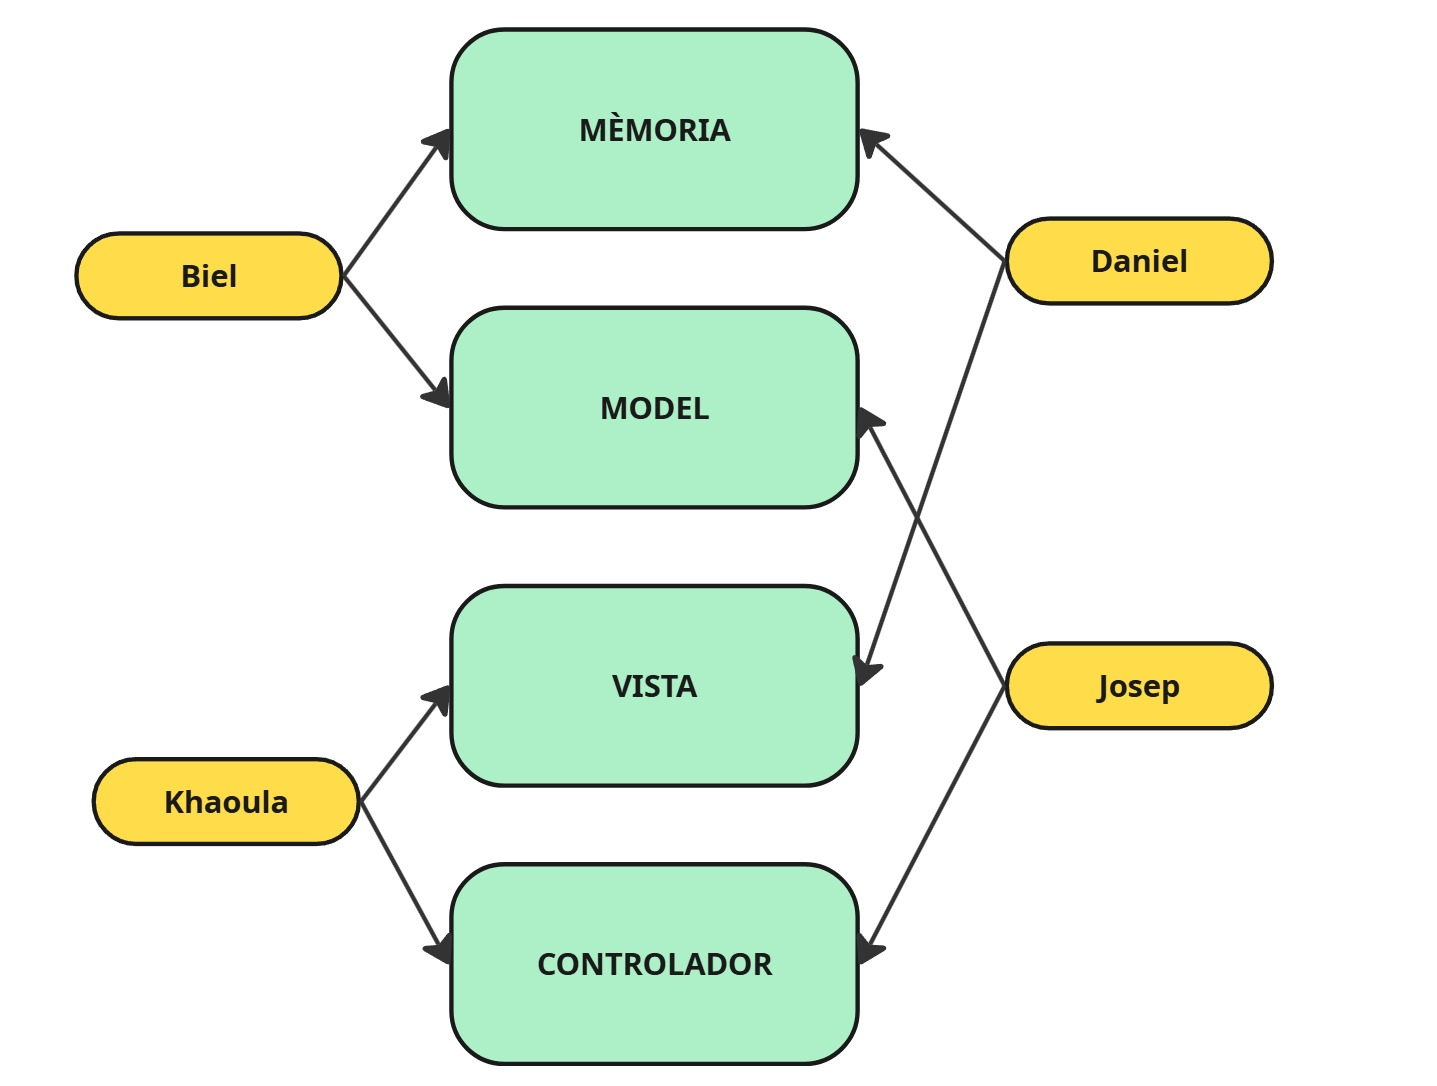
\includegraphics[width=0.45\textwidth]{docs/png/repartiment.jpg}}
    \caption{Repartiment de feina}
    \label{fig:distMin}
\end{figure}

Tot i que la figura mostra una aparença d'independència en la distribució de les tasques entre els membres de l'equip, la realitat va ser diferent. Alguns membres van acabar intervenint en àrees que no els havien estat assignades originalment, ja sigui corregint errors o afegint funcionalitats addicionals.


\begin{thebibliography}{9}

\bibitem{bigOAnalysis}
GeeksforGeeks. (2021). \textit{Analysis of Algorithms | Big-O Analysis}. Recuperat de: \url{https://www.geeksforgeeks.org/analysis-algorithms-big-o-analysis/}

\bibitem{Patró per Esdeveniments} 
Eric Gamma, Richard Helm, Ralph Johnson, and John Vlissides. \emph{Design Patterns: Elements of Reusable Object-Oriented Software}. Addison-Wesley, 1994.

\bibitem{JavaFX}
OpenJFX, \textit{The official home of JavaFX}.  
\url{https://openjfx.io/},  

\bibitem{MVC_Theory}
Trygve Reenskaug, "The Model-View-Controller (MVC) Pattern," \textit{Software Engineering Notes}, vol. 10, no. 6, pp. 1-3, Dec. 1985. [En línia]. Disponible: \url{https://en.wikipedia.org/wiki/Trygve_Reenskaug}.

\bibitem{closestPairTheory}
Wikipedia, \textit{Closest pair of points problem}, \url{https://en.wikipedia.org/wiki/Closest_pair_of_points_problem}, Accés: 2025-04-15


\bibitem{MVCPattern}
GeeksforGeeks. (2021). \textit{MVC Design Pattern}. Recuperat de: \url{https://www.geeksforgeeks.org/mvc-design-pattern/}

\bibitem{mvcBenefits}
GeeksforGeeks. (2021). \textit{Benefit of Using MVC}. Recuperat de: \url{https://www.geeksforgeeks.org/benefit-of-using-mvc/}

\bibitem{SwingLibrary}
Oracle, "Swing: A GUI Widget Toolkit," \textit{Oracle Documentation}, Oracle Corporation, 2009. [En línia]. Disponible: \url{https://docs.oracle.com/javase/8/docs/api/javax/swing/package-summary.html}.

\bibitem{oracleExecutorService}
Oracle. (2014). \textit{ExecutorService Interface (Java Platform SE 8)}. Recuperat de: \url{https://docs.oracle.com/javase/8/docs/api/java/util/concurrent/ExecutorService.html}

\bibitem{DivideAndConquer}
Wikipedia (Español), \textit{Algoritmo divide y vencerás}.  
\url{https://es.wikipedia.org/wiki/Algoritmo_divide_y_vencer%C3%A1s#:~:text=En%20la%20cultura%20popular%2C%20divide,las%20partes%20se%20torna%20obvia},  

\bibitem{kdTree}
Wikipedia (Francès), \textit{Arbre kd}.  
\url{https://fr.wikipedia.org/wiki/Arbre_kd},  

\bibitem{GrahamScan}
\textit{An efficient algorith for determining the convex hull of a finite planar set}, \url{https://mathweb.ucsd.edu/~ronspubs/72_10_convex_hull.pdf}, 

\bibitem{quickhull}
Wikipedia, \textit{Quickhull}, \url{https://en.wikipedia.org/wiki/Quickhull}

\bibitem{John}
QuickHull3D: A Robust 3D Convex Hull Algorithm in Java
\url{https://www.cs.ubc.ca/~lloyd/java/quickhull3d.html}

\bibitem{singleton}
Wikipedia, \textit{Singleton Pattern} \url{https://en.wikipedia.org/wiki/Singleton_pattern}


\bibitem{rosebrock}
Adrian Rosebrock, \textit{Implementing Approximate Nearest Neighbor Search with KD-Trees}, \url{https://pyimagesearch.com/2024/12/23/implementing-approximate-nearest-neighbor-search-with-kd-trees/}

\bibitem{youtube}
William Fiset, \textit{K-D Trees - Data Structures}, YouTube, \url{https://www.youtube.com/watch?v=ivdmGcZo6U8}

\bibitem{mdpi}
Yu-Chi Lu et al., \textit{Air Pollution Exposure and Health Outcomes: A Review from the Epidemiologic Perspective}, International Journal of Environmental Research and Public Health, \url{https://www.mdpi.com/1660-4601/11/9/9101}
\end{thebibliography}
\end{document}


